\documentclass[11pt, aspectratio=149]{beamer}
% xcolor=dvipsnames option for more colors...

\usepackage[export]{adjustbox}
%\usepackage{wrapfig}
%\usepackage{subfigure}
%\usepackage{bbm}
\usepackage{amssymb}
\usepackage{amsmath}
\usepackage{amsthm}

\newtheorem{claim}{Claim}
\newtheorem{prop}{Proposition}
\newtheorem{lem}{Lemma}
\newtheorem{conj}{Conjecture}
\newtheorem{cor}{Corollary}


\newcommand{\Rm}{\mathbb{R}}
\newcommand{\Zm}{\mathbb{Z}}
\newcommand{\Qm}{\mathbb{Q}}

\newcommand{\Pc}{\mathcal{P}}
\newcommand{\Hc}{\mathcal{H}}
\newcommand{\Ec}{\mathcal{E}}
\newcommand{\Qc}{\mathcal{Q}}
\newcommand{\Nc}{\mathcal{N}}
\newcommand{\RGc}{\mathcal{RG}}
\newcommand{\STc}{\mathcal{ST}}
\newcommand{\Wc}{\mathcal{W}}
\newcommand{\Mc}{\mathcal{M}}
\newcommand{\Lc}{\mathcal{L}}
\newcommand{\PSc}{\mathcal{PS}}
\newcommand{\Gc}{\mathcal{G}}
\newcommand{\Fc}{\mathcal{F}}
\newcommand{\Tc}{\mathcal{T}}

\renewcommand{\u}{\underline}
\newcommand{\kkappa}{\underline{\kappa}}
\newcommand{\kk}{\underline{k}}
\newcommand{\vp}{\operatorname{vp}}

\renewcommand{\b}{^{\bullet}} %ATTENTION REDEFINED COMMAND
\newcommand{\w}{^{\circ}}
\newcommand{\sqb}{{\blacksquare}}
\newcommand{\sqw}{{\square}}
\newcommand{\pp}{\pi} % prefix-postfix sequence of a tree

\newcommand{\dgu}{{\underline{k}}}
\newcommand{\dg}{{k}}
\newcommand{\Vol}{\operatorname{Vol}}
\newcommand{\cVol}{\operatorname{\overline{Vol}}}
\newcommand{\cQ}{\mathcal{Q}}
\newcommand{\cH}{\mathcal{H}}

\usepackage{array}

\title[Audition MCF P13/LIPN]{Audition MCF P13/LIPN}
\author[Ivan Yakovlev]{Ivan Yakovlev}
\institute[MPIM]{}
\date[13 Mai 2026]{}


% \AtBeginSection[]{
%   \begin{frame}{Outline}
%     \tableofcontents[currentsection]
%   \end{frame}
% }

\usecolortheme[named=purple]{structure}
\usetheme{Madrid}
\usecolortheme{dolphin}

\usefonttheme{professionalfonts}
%\useinnertheme{circles}
\beamertemplatenavigationsymbolsempty

\setbeamertemplate{page number in head/foot}[appendixframenumber]

\usepackage[labelformat=empty,justification=centering]{caption}

% \newcommand{\nb}[1]{
% \begin{flushright} 
% \color{red} \tiny{#1}
% \end{flushright}
% }

\begin{document}

\frame{
\titlepage
\vspace{-2cm}
\begin{table}
	\footnotesize 
	\centering 
	\begin{tabular}{l l}
		2024 -- 2026 & Postdoc (MPI for Mathematics, Bonn) \\
		2021 -- 2024 & Doctorat (LaBRI, Bordeaux) \\
		2018 -- 2021 & ENS + M2 Math Fonda (Paris) \\
		2015 -- 2019 & Licence Math Appli (Kiev)	
	\end{tabular}
\end{table}
}

\begin{frame}{Enseignement : expérience}
	
2021 -- 2024, Université de Bordeaux, Licence Info.
    \smallskip
\begin{table}
\centering
    \begin{tabular}{|m{0.03\textwidth}|m{0.5\textwidth}|m{0.04\textwidth}|m{0.12\textwidth}|}
    \hline
    	L1 & Initiation à la programmation C & 32h & CI/TDM \\ \hline
    	L1 & Algorithmique des tableaux (Python) & 32h & TDM \\ \hline
    	L2 & Algorithmique des structures de données arborescentes (OCaml) & 32h & CI/TDM \\ \hline
    	L2 & Probabilités, Statistiques et Combinatoire & 28h & TD \\ \hline
    	L2 & Réseaux & 32h & TD/TDM  \\ \hline
    	
        %L1 & Initiation à la \alert{programmation} C & 32h & CI/TDM \\ \hline
    	%L1 & \alert{Algorithmique} des tableaux (Python) & 32h & TDM \\ \hline
    	%L2 & \alert{Algorithmique} des structures de données arborescentes (OCaml) & 32h & CI/TDM \\ \hline
        %L2 & \alert{Probabilités, Statistiques et Combinatoire} & 28h & TD \\ \hline
    	%L2 & \alert{Réseaux} & 32h & TD/TDM  \\ \hline
    \end{tabular}
\end{table}

%\alert{Intégration enseignement}:  encadrement.

\end{frame}

\begin{frame}{Enseignement : projet d'intégration}
	\textbf{Dès la rentrée} : 
	\begin{itemize}
		\item programmation impérative/fonctionnelle/orientée objet, réseaux, algorithmique, automates/langages, proba/stats;
		\item encadrement;
	\end{itemize}
	\textbf{\'{A} court terme} :
	\begin{itemize}
		\item architecture, administration, systèmes d'exploitation, programmation web, bases de données;
		\item responsabilité d'année.
	\end{itemize}
 \end{frame}


\begin{frame}{Activités diverses}
\begin{tabular}{p{0.13\textwidth} p{0.8\textwidth}}
    \alert{Organisation} & 
    \begin{itemize}
        \item séminaire de l'équipe ``Combinatoire et Interactions'' (Bordeaux, 2022 -- 2023)
        \item école ``Surfaces plates et interactions'' (Le Teich, 2024)
        \item groupe de lecture ``Géométrie spectrale'' (Bonn, 2026)
    \end{itemize}\\ 
     \vspace{-5mm} \alert{Diffusion} & 
     \vspace{-5mm} 
     \begin{itemize}
         \item enseignement des mathématiques olympiques aux collégiens et lycéens (Kiev 2015 -- 2018, Marseille 2022)
         \item organisation / jury aux olympiades mathématiques \\ (Kiev 2015 -- 2018, EGMO 2019)
     \end{itemize}\\
\end{tabular}    
\end{frame}

\begin{frame}{Recherche}
    \begin{figure}
        \centering
        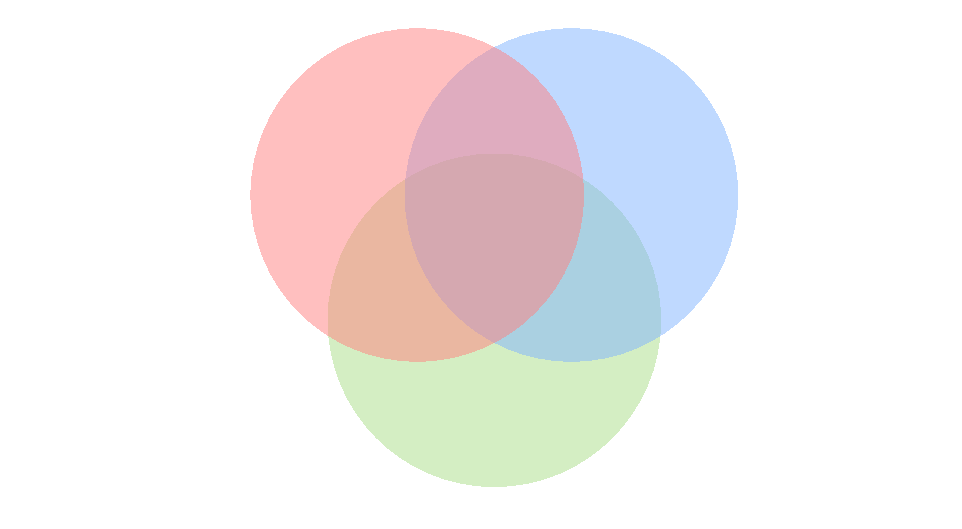
\includegraphics[width=0.8\linewidth]{circles.pdf}
    \end{figure}
\end{frame}

\begin{frame}{Travaux}
    \begin{enumerate}
        \item I. Yakovlev, \emph{Contribution of $n$-cylinder square-tiled surfaces to Masur–-Veech volume of $\Hc(2g-2)$}, \textbf{GAFA} (2023).
        \item V.Delecroix, M.Ebbens, F.Lazarus, I.Yakovlev, \emph{Algorithms for Length Spectra of Combinatorial Tori}, \textbf{SoCG 2023}, \textbf{JoCG} (2024).
        \item I.Yakovlev, \emph{Metric ribbon graphs}, \textbf{thèse de doctorat} (2024).
        \item E. Duryev, É. Goujard, I. Yakovlev, \emph{Volumes of odd strata of quadratic differentials}, \textbf{soumis} (2025).
    \end{enumerate}
\end{frame}

\begin{frame}{Surfaces de translation}
    \begin{figure}

        \centering
        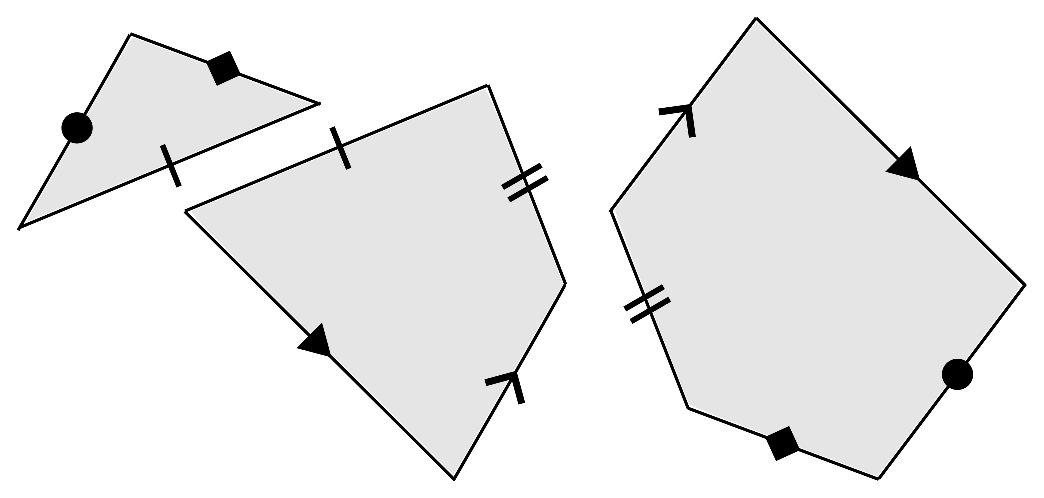
\includegraphics[width=0.4\linewidth]{euclidean-polygons.eps}
        \hspace{15mm}
        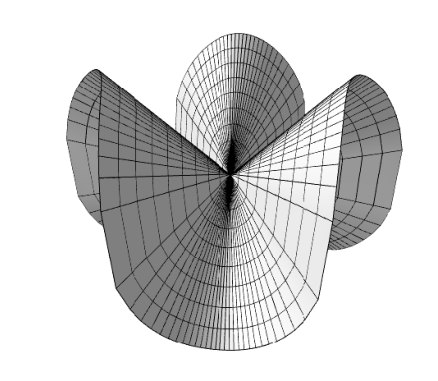
\includegraphics[width=0.23\linewidth]{singularity.eps}
    \end{figure}

    %Trois définitions équivalentes :
{ \centering
\alert{Recollement de polygones} le long de cotés égaux et parallèles.

$\Updownarrow$
  
\alert{Surface plate} aux singularités coniques d'angles $2\pi k$ (et l'holonomie triviale).
}
        %\item courbe complexe muni d'une 1-forme holomorphe (\alert{différentielle abélienne}).
\end{frame}

\begin{frame}{Espaces de modules (paramètres)}

\alert{Strates des surfaces de translation :} 
\[\Hc(\u k) = \Hc(k_1,\ldots, k_n) = \left \{
\begin{array}{c}
     \text{surfaces de translation aux} \\ 
     \text{angles coniques $2\pi(k_i+1)$}
\end{array}\right \}\]

\begin{itemize}
	\item variétés (localement $\mathbb{R}^n$);
	\item  coordonnées : vecteurs des cotés des polygones;
	\item admettent une mesure finie naturelle (\alert{mesure de Masur--Veech}).
\end{itemize}


%\bigskip
%$\leadsto$ constantes de Siegel--Veech (Eskin-Masur-Zorich '03, Goujard '15) \\ \quad \ exposants de Lyapunov (Eskin-Kontsevich-Zorich '14) 

%$\leadsto$ comptage de géodésiques sur les surfaces plates (Eskin-Masur '01) \\ \quad \ taux de diffusion des billards périodiques (Delecroix-Hubert-Lelièvre '14)

\end{frame}

\begin{frame}{Surfaces à petits carreaux (SPC)}

\[\text{Calcul des volumes de Masur--Veech} \iff \begin{array}{c}\text{\alert{énumération asymptotique} des} \\ \text{``points entiers'' dans les strates.}\end{array}\]

\vspace{3mm}
    
        \begin{minipage}{0.3\linewidth}
        \begin{figure}
        \centering
            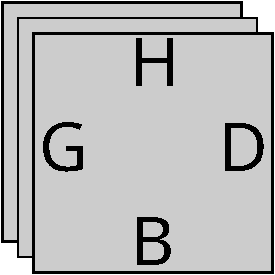
\includegraphics[width=0.5\linewidth]{squares-french.pdf}
            \caption{Règle de recollement :\\ $H \leftrightarrow B$, $G \leftrightarrow D$}
        \end{figure}
        \end{minipage}%
        \begin{minipage}{0.69\linewidth}
        \vspace{-1cm}
        \begin{figure}
        \centering
            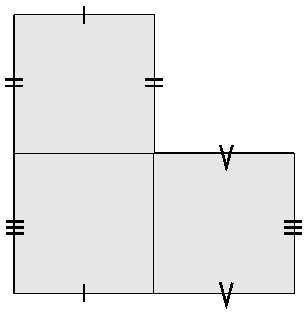
\includegraphics[height=0.3\textheight]{4-2.pdf}
            \hspace{5mm}
            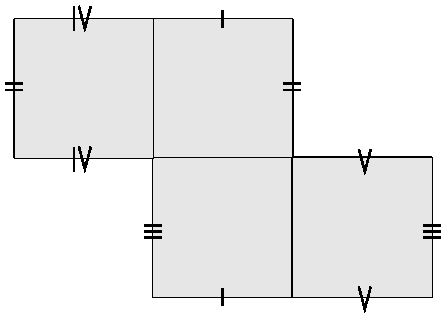
\includegraphics[height=0.3\textheight]{4-3.pdf}
        \end{figure}
        \end{minipage}
        % \vspace{1mm}
        % \[\# \{\text{SPC dans $\Hc(\u k)$ avec $\le N$ carreaux}\} \sim \operatorname{const} \cdot \alert{\operatorname{Vol} \Hc(\u k)} \cdot N^{2g+n-1},\ N \rightarrow \infty\]
    
\end{frame}

\begin{frame}{Approches aux volumes de Masur--Veech}

Théorie des représentations des groupes symétriques (Eskin-Okounkov '01), théorie de l'intersection (Sauvaget '18, Chen-M\"{o}ller-Sauvaget-Zagier '20),
\alert{approche combinatoire} (Athreya-Eskin-Zorich '14, Delecroix-Goujard-\\-Zograf-Zorich '21).

\pause

%\vspace{3mm}
    \begin{center}
        SPC = cylindres + \alert{graphes en rubans métriques}
    \end{center}
    \begin{figure}
        \centering
        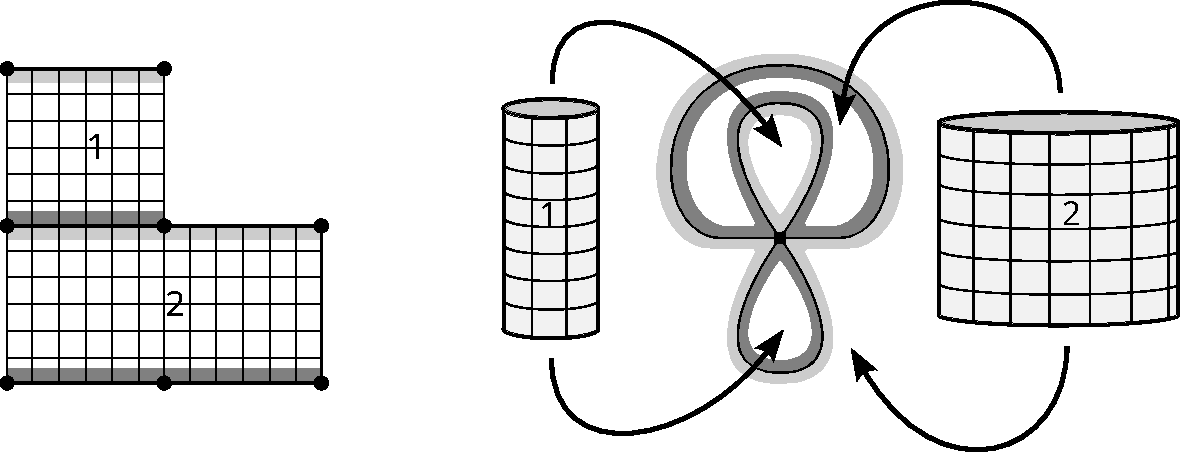
\includegraphics[width=0.65\linewidth]{cyl-decomp.pdf}
        %\vspace{3mm}
        %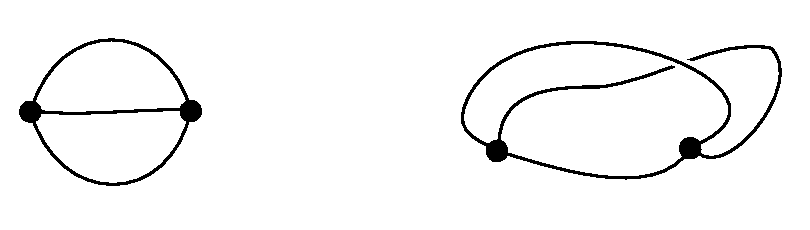
\includegraphics[width=0.5\textwidth]{def-rg-1.pdf}
    \end{figure}
\end{frame}

\begin{frame}{Comptage de graphes en rubans métriques}

$\leadsto$ compter les graphes en rubans métriques de genre $g$ avec $n$ bords de longueurs $L_1,\ldots,L_n$.

\pause
    \begin{block}{Théorème (Kontsevich '92)}
        Graphes \alert{trivalents} $\Rightarrow$ \alert{polynôme} en $L_i$ dont les coefficients sont les nombres d'intersection $\int_{\overline{\Mc}_{g,n}} \psi_1^{d_1}\cdots \psi_n^{d_n}$.
    \end{block}
    \pause
    \begin{block}{Théorèmes}
    Fonctions de comptage \alert{polynomiales} explicites :\\
    \begin{itemize}
        \pause \item \textbf{(Y. '23)} Graphes \alert{face-bicolores à un sommet}.
        \pause \item \textbf{(Y. '24)} Comptage pondéré des graphes \alert{face-bicolores à $\ge 2$ sommets}.
        \pause \item \textbf{(Duryev-Goujard-Y. '25)} Graphes aux \alert{degrés de sommets impaires fixés}.
    \end{itemize}        
    \end{block}
    
\end{frame}


\begin{frame}{Outils : combinatoire bijective}
    
    \textbf{(Y. '23)} : \alert{bijection de Chapuy-Féray-Fusy '13} entre les graphes en rubans à un bord et les arbres planes décorés.

    \textbf{(Y. '24)} : \alert{bijection de Bernardi '07} entre les graphes planaires munis d'un arbre couvrant et les paires d'arbres planaires.

    \textbf{(Duryev-Goujard-Y. '25)} : \alert{bijection à la Pr\"{u}fer} pour les arbres étiquetés.
    
    \begin{figure}
        \centering
        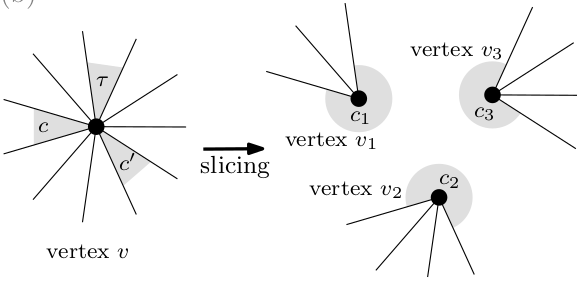
\includegraphics[width=0.3\textwidth]{chapuy-2.png}
        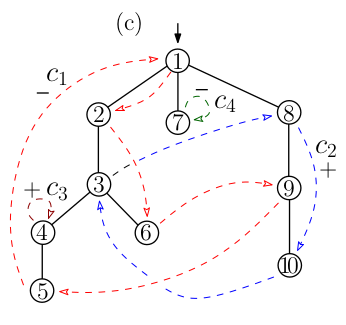
\includegraphics[width=0.2\textwidth]{chapuy-3.png}
        \hspace{0.05\textwidth}
        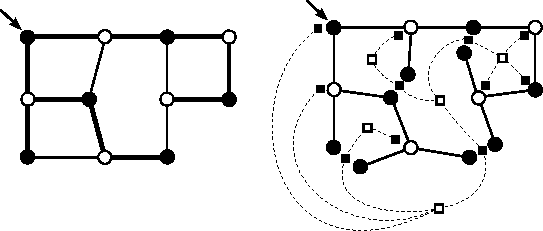
\includegraphics[width=0.4\textwidth]{many-vertices-bij-bis.pdf}
    \end{figure}
\end{frame}


\begin{frame}{Applications}

    \begin{block}{Théorème (Y. '23)}
    Formule explicite pour la série génératrice bivariée $\mathcal{C}(t,u)$ des contributions $a_{g,n}$ des surfaces à petits carreaux avec $n$ cylindres au \alert{volume de $\Hc(2g-2)$}.
    \end{block}
    % \begin{block}{Théorème (Y. '23)}
    % Soit $a_{g,n}$ la contribution (normalisée) des surfaces à petits carreaux avec $n$ cylindres au \alert{volume de $\Hc(2g-2)$} et soit $\mathcal{C}(t,u) = 1 + \sum_{g\geq 1} \left(\sum_{n=1}^g a_{g,n} u^n \right) (2g-1)t^{2g}$. Alors pour tout $g\geq 0$
    %     \begin{equation*}
    %         \label{eq:relation_bivariate}
    %         \frac{1}{(2g)!} [t^{2g}] \mathcal{C}(t,u)^{2g} = [t^{2g}] \left(\frac{t/2}{\sin(t/2)}\right)^u.
    %     \end{equation*}
    % \end{block}
	$\leadsto$ distribution des cylindres des SPC aléatoires dans $\Hc(2g-2)$ (travail en cours)

    %\begin{itemize}
        %\item inversion de Lagrange $\Rightarrow$ formule explicite pour $\mathcal{C}(t,u)$;
        %\item $u=1 \Rightarrow$ formule de Sauvaget '18 pour les volumes totaux, obtenu par la géométrie algébrique %$\leadsto$ interprétation algébrique de $\mathcal{C}(t,u)$ ?
        %\item $a_{g,n}/\sum_k a_{g,k}$ -- proba qu'une SPC aléatoire dans $\Hc(2g-2)$ a $n$ cylindres.
    %\end{itemize}
\medskip
\pause
    \begin{block}{Théorème (Duryev-Goujard-Y. '25)}
    Récursion explicite pour les \alert{volumes des strates de différentielles quadratiques aux singularités impaires}, qui fait intervenir les nombres d'intersection des classes psi et les cycles combinatoires de Kontsevich--Witten.
    \end{block}
	$\leadsto$ asymptotique des volumes pour $g \rightarrow \infty$ (travail en cours)
\end{frame}

\begin{frame}{Projet de recherche}
	
	\begin{figure}
		\centering
		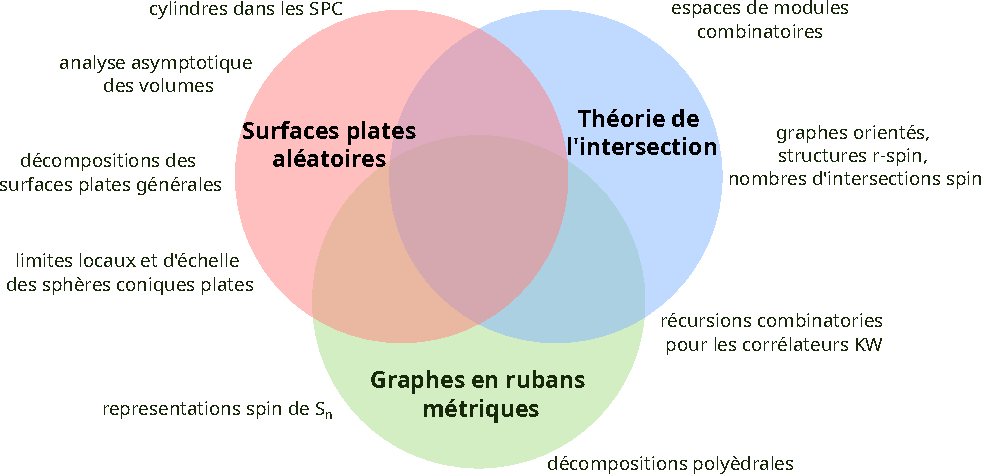
\includegraphics[width=0.9\linewidth]{circles-2.pdf}
	\end{figure}
	
    %\begin{itemize}
       %\item \alert{statistiques explicites} des cylindres pour les strates plus générales et leurs composantes connexes;
       %\item \alert{distributions asymptotiques} des nombres de cylindres (conjectures de Delecroix-Goujard-Zograf-Zorich);
       %\item \alert{phénomène de polynomialité} pour les fonctions de comptage;
       %\item \alert{combinatoire des polynômes de Kontsevich} et des nombres d'intersection (orientations de Kasteleyn, structures spin, formules locales combinatoires);
       %\item interprétation des résultats combinatoires par la \alert{géométrie algébrique / théorie des représentations}.
    %\end{itemize}
\end{frame}

\begin{frame}{Intégration}
\begin{itemize}
	\item Thierry Monteil (surfaces de translation);
	\item Meltem Ünel (limites locaux/globaux d'arbres, des cartes combinatoires, géométrie hyperbolique);
	\item Lionel Pournin (géométrie polyèdrale, graphes des flips);
	\item Andrea Sportiello (systèmes intégrables, modèles de mécanique statistique);
	\item Axel Bacher, Cyril Banderier, Frédérique Bassino (combinatoire énumérative).
\end{itemize}
\end{frame}

\appendix

\section{Slides cachés}

  \begin{frame}
  \vfill
  \centering
    \usebeamerfont{title}\usebeamercolor[fg]{title}\insertsectionhead\par%
  \vfill
  \end{frame}

\begin{frame}{Computing degeneration coefficients on the walls}
            \begin{figure}
            \centering
            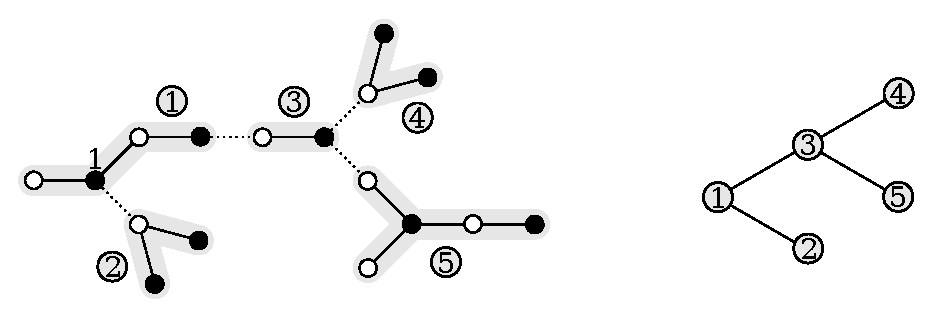
\includegraphics[width=0.8\textwidth]{degenerate-tree-new.eps}
           
        \end{figure}

         \begin{equation*}
    \label{eq:pNumbersRecursion}
    (k+l-2)! = p^{b_1,\ldots,b_n}_{w_1,\ldots,w_n} + \sum_{t=2}^n \frac{\color{red}(k+l-2)_{t-2}}{t!} \sum_{I_1, \ldots I_t} \prod_{j=1}^t \left(\sum_{i\in I_j} (b_i+w_i) - 1\right) p^{b_{I_j}}_{w_{I_j}},
    \end{equation*}
\end{frame}

\begin{frame}{Degenerations in the quadratic case}
\begin{figure}
    \centering
    \def\svgwidth{0.55\textwidth}
    \input{odd-joining-to-markers.pdf_tex}
    
\end{figure}

    {\tiny 
    A joining is admissible if and only if for every $i=1,\ldots, m$ the following holds:
\begin{itemize}
    \item if all of the descendants of $G_i$ have labels smaller then $i$, then the bridge joining $G_i$ to its parent is in the black corner of $G_i$;
    \item otherwise, the bridge joining $G_i$ to its parent and the bridge joining $G_i$ to the subtree containing the descendant of $G_i$ of maximal label are in the corners of $G_i$ of different colors.
\end{itemize}
    }
\end{frame}

\begin{frame}{Cylinder contributions in $\Hc(2g-2)$}
    \begin{theorem}[Y., 2023]
    The contribution of $n$-cylinder square-tiled surfaces to the volume of $\Hc(2g-2)$ is equal to $\frac{2(2\pi)^{2g}}{(2g-1)!}a_{g,n}$, where $a_{g,n} \in \Qm$, and whose generating function $\mathcal{C}(t,u) = 1 + \sum_{g\geq 1} \left(\sum_{n=1}^g a_{g,n} u^n \right) (2g-1)t^{2g}$ satisfies for all $g\ge 0$
    \[
    \frac{1}{(2g)!} [t^{2g}] \mathcal{C}(t,u)^{2g} = [t^{2g}] \left(\frac{t/2}{\sin(t/2)}\right)^u.
    \]
    \end{theorem}
    \begin{itemize}
        \pause \item Lagrange inversion $\Rightarrow$ explicit formula for $\mathcal{C}(t,u)$;
        \pause \item setting $u=1$ we recover the result of Sauvaget.
        \pause \item Faber-Pandharipande 2000: $\left(\frac{t/2}{\sin(t/2)}\right)^{u+1}$ is the generating function of Hodge integrals $\int_{\overline{\mathcal{M}}_{g,1}} \lambda_{g-i} \psi_1^{2g-2+i}$
    \end{itemize}
\end{frame}


\begin{frame}{Cylinder contributions in spin components of $\Hc(2g-2)$}
\begin{theorem}[Y., 2024+]
    The difference of the contributions of $n$-cylinder square-tiled surfaces to the volumes of even and odd spin subspaces of $\mathcal{H}(2g-2)$ is equal to $\frac{2(2\pi i)^{2g}}{(2g-1)!}d_{g,n}$, where $d_{g,n} \in \mathbb{Q}$, and whose generating function
        $\mathcal{D}(t,u) = 1 + \sum_{g\geq 1} \left(\sum_{n=1}^g d_{g,n} u^n \right)(2g-1) t^{2g}$
        satisfies for all $k\geq 1$
        \begin{equation*}
        \label{eq:spin-D-series-relation}
            \frac{1}{2k} [t^{2k}] \mathcal{D}(t,u)^{2k} = \frac{B_{2k}}{2^{k+1} k} u,
        \end{equation*}
    where $B_{2k}$ is the $2k$-th Bernoulli number.
\end{theorem}

\pause $u=1$ : formula from Chen, M\"{o}ller, Sauvaget, Zagier.
\end{frame}

\begin{frame}{Ribbon graphs ($=$ combinatorial maps)}

A \alert{ribbon graph} is a graph (loops and multiple edges allowed) with a circular ordering of (half-)edges incident to every vertex.

\begin{figure}
    \begin{overprint}
    
        \onslide<1-2> 
        \centering 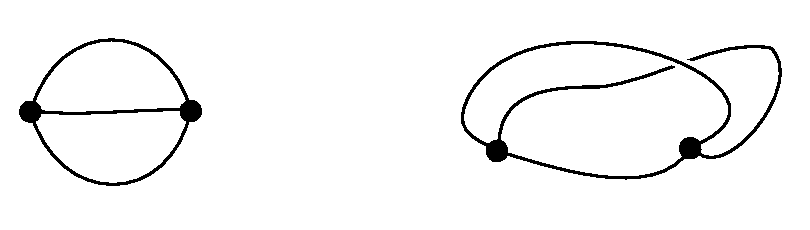
\includegraphics[width=0.8\textwidth]{def-rg-1.pdf}
        \onslide<3> 
        \centering 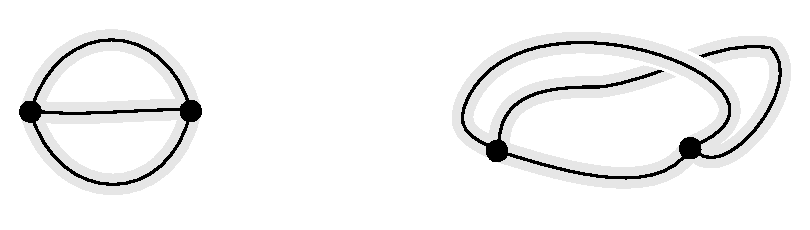
\includegraphics[width=0.8\textwidth]{def-rg-2.pdf}
        \onslide<4-> 
        \centering 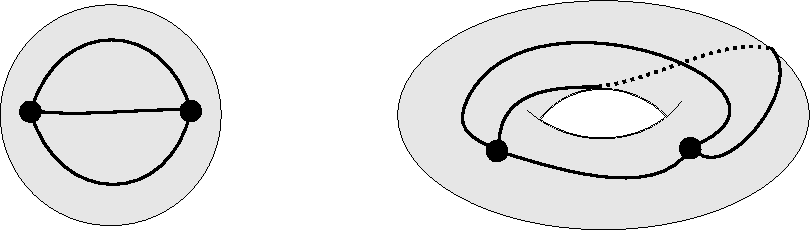
\includegraphics[width=0.8\textwidth]{def-rg-3.pdf}
    \end{overprint}
\end{figure}

\pause
Equivalently, cellular embedding of a graph into a surface. \smallskip

\pause \pause \pause
\alert{Euler's formula}: $|V(G)|-|E(G)|+|F(G)| = 2-2g$.\smallskip

%\pause

%A \alert{metric} on a ribbon graph $G$ is a function $E(G) \rightarrow \Rm_{>0}$. 

\end{frame}


% \begin{frame}{Enumeration of ribbon graphs (\emph{pot-pourri})}

% \begin{itemize}
%     \item \textbf{Tutte '63} (\emph{equations with catalytic variable}): number of planar maps with $n$ edges is equal to $\frac{2\cdot 3^n (2n)!}{n!(n+2)!}$.
%     \item \textbf{Harer-Zagier '86} (\emph{matrix integrals}): generating series for one-face maps is equal to $\left(\frac{1+x}{1-x} \right)^y$.
%     \item \textbf{Goulden-Jackson '08} (\emph{representation theory of $S_n$}): generating series of maps satisfies the Kadomtsev-Petviashvili (KP) hierarchy of PDEs.
%     \item \textbf{Chassaing-Schaeffer '04} (\emph{bijections with decorated trees}): diameter of a random planar quadrangulation with $n$ faces is of order $n^{1/4}$.
%     \item \textbf{Le Gall, Miermont '13}: let $Q_n$ be a uniformly random planar quadrangulation with $n$ faces; then, as $n \rightarrow \infty$,
%     \begin{equation*}
%         (Q_n , d_{graph} \cdot n^{-1/4}) \longrightarrow \text{Brownian sphere}.
%     \end{equation*}
% \end{itemize}
% \end{frame}

% \begin{frame}{Families of ribbon graphs}
%     For $g \ge 0$, $n \ge 1$ and $d$ a partition, let
%     \begin{equation*}
%         \RGc^d_{g,n} = \left \{
%         \begin{array}{c}
%            \text{genus } g \text{ ribbon graphs with } n \text{ \emph{labeled} boundary}\\
%            \text{ components and vertex degrees given by } d
%         \end{array}
%         \right \}
%     \end{equation*}

%     For $k,l\ge 1$, let 
%     \begin{equation*}
%         \RGc^d_{g,(k,l)} = \left \{
%         \begin{array}{c}
%            \text{genus } g \text{ \alert{face-bicolored} ribbon graphs with } k \text{ black and } l \text{ white}\\
%            \text{ \emph{labeled} boundary components and vertex degrees given by } d
%         \end{array}
%         \right \}
%     \end{equation*}
    
%     $\RGc_{g,n}$, $\RGc_{g,(k,l)}$ -- no constraints on vertex degrees.
% \end{frame}

\begin{frame}{Metric ribbon graphs and counting functions}
    A \alert{metric} on a ribbon graph $G$ is a function $E(G) \rightarrow \Rm_{>0}$. \smallskip

    \pause
    For a ribbon graph $G$ with $n$ labeled faces and $L_1,\ldots,L_n \in \Zm$, let
    \begin{equation*}
        \Nc_G(L_1,\ldots, L_n) = 
        \# \left \{
        \begin{array}{c}
             \text{\emph{integer} metrics on } G \text{ with \alert{perimeter} of}\\
             \text{the } i\text{-th face equal to } L_i
        \end{array}
        \right \}
    \end{equation*}

    \pause
    For a \emph{face-bicolored} ribbon graph $G$ with $k$ black and $l$ white faces, and $L_1,\ldots,L_k, L'_1,\ldots,L'_l \in \Zm$, define analogously
    \begin{equation*}
        \Nc_G(L_1,\ldots, L_k; L'_1,\ldots,L'_l).
    \end{equation*}
    % \begin{equation*}
    %     \Pc_G(L_1,\ldots, L_n; L'_1,\ldots,L'_l) = 
    %     \# \left \{
    %     \begin{array}{c}
    %          \text{\emph{integer} metrics on } G \text{ with \alert{perimeter} of}\\
    %          \text{the } i\text{-th boundary component equal to } L_i
    %     \end{array}
    %     \right \}
    % \end{equation*}
\end{frame}

\begin{frame}{Computing a counting function}
\begin{figure}
    \begin{overprint}
        \onslide<1-2>
        \centering
        \def\svgwidth{0.4\textwidth}
        \input{intro-5-0.pdf_tex}
        \onslide<3->
        \centering
        \def\svgwidth{0.4\textwidth}
        \input{intro-5-1.pdf_tex}
    \end{overprint}
    
\end{figure}

\pause
$\Nc_G$ is zero outside of $\left \{ \sum_i L_i = \sum_j L'_j,\ L_i>0,\ L'_j>0 \right \}$.
\begin{equation*}
\pause \pause
    \begin{cases}
    a,b,c,d > 0\\
    a=L_1\\
    b+c+d=L_2\\
    a+b=L'_1\\
    c+d=L'_2
    \end{cases}
\pause
    \iff \ \ 
    \begin{cases}
    a,b,c,d > 0\\
    a=L_1\\
    b=L'_1-L_1\\
    c+d=L'_2
    \end{cases}
\pause
    \Rightarrow \Nc_G(L;L') = \mathbf{1}_{L'_1 > L_1} \cdot (L'_2-1).
\end{equation*}
\end{frame}

\begin{frame}{Counting functions}
%Let $\PSc_{k,l}$ be the polyhedral subdivision of $\Rm^k \times \Rm^l$ generated by the hyperplanes (``walls'') of the form $\sum_{i \in I} L_i = \sum_{j \in J} L'_j,\ I \subset \{1,\ldots,k\},\ J \subset \{1, \ldots, l\}$.

%\pause
    \begin{block}{Proposition}
        For any $G$ the function $\Nc_G$ is \alert{piecewise {\tiny (quasi-)}polynomial}. The regions of polynomiality are cut out by a certain hyperplane arrangement $\Hc_n$ ($\Hc_{k,l}$).
    \end{block}

\pause
Idea of proof: counting integer points in a deforming polytope.
 \begin{figure}
    \centering
    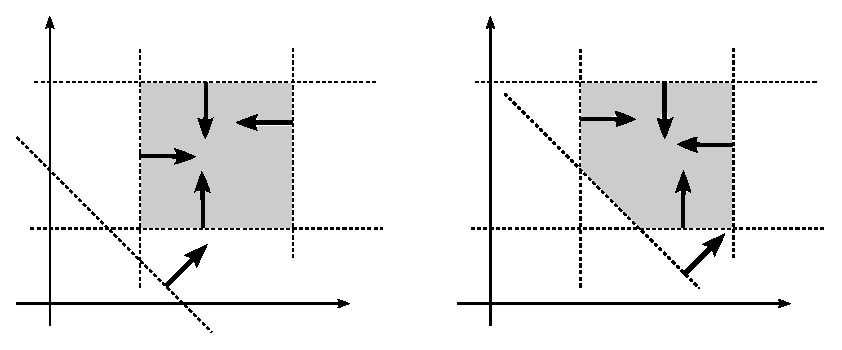
\includegraphics[height=0.25\textheight]{polytopes.eps}
\end{figure}
\pause
Note that the \alert{top-degree term} of $\Nc_G$ gives the \alert{volume} of this polytope!

\end{frame}

\begin{frame}{Counting functions}

Introduce the counting functions for families $\RGc^d_{g,n}$ of ribbon graphs sharing the same genus $g$, number of faces $n$ and vertex-degree profile $d$:
\begin{align*}
    \Nc^d_{g,n}(L) &= \sum_{G \in \RGc^d_{g,n}} \frac{1}{|\operatorname{Aut}(G)|}\cdot \Nc_G(L). %,\\
    %\Nc^d_{g,(k,l)}(L,L') &= \sum_{G \in \RGc^d_{g,(k,l)}} \frac{1}{|\operatorname{Aut}(G)|}\cdot \Nc_G(L,L').
\end{align*}

\pause 
Define $\Nc^d_{g,(k,l)}(L,L')$ analogously.

\pause
\bigskip
\centering
\emph{A priori} piecewise (quasi-)polynomials... 
\pause 

But \alert{sometimes the top-degree term is polynomial!}
\end{frame}

\begin{frame}{Example 1: trivalent graphs}

Consider the families of \emph{trivalent} ribbon graphs: $d = [3,\ldots, 3] = [3^{4g+2n-4}]$.

\pause
\begin{block}{Theorem (Kontsevich, '92)}
    For any $g,n$, the \alert{top-degree term} of $\Nc^{[3^{4g+2n-4}]}_{g,n}$ is a \alert{polynomial}
    % \begin{equation*}
    %     \frac{1}{2^{{5g-6+2n}}} \sum_{d_1+\ldots+d_n = 3g-3+n} \langle \tau_{d_1}\cdots \tau_{d_n} \rangle \prod_{i=1}^n \frac{L_i^{2d_i}}{d_i!},
    % \end{equation*}
    whose coefficients are the intersection numbers of $\psi$-classes on the moduli space of marked Riemann surfaces: $ \int_{\overline{\Mc}_{g,n}} \psi_1^{\alpha_1}\cdots \psi_n^{\alpha_n}$.
\end{block}

\pause
\bigskip
Idea: polytopes corresponding to all graphs $G$ can be glued together to form a space homeomorphic to $\overline{\Mc}_{g,n}$.
% \pause
% \textbf{Norbury '10}: $\Nc^{[3^{4g+2n-4}]}_{g,n}$ is a quasi-polynomial. \smallskip
% \pause 

% Witten's conjecture, $\Mc^{comb}_{g,n}$, Weil-Petersson volumes (\textbf{Mirzakhani '08}).
\end{frame}

% \begin{frame}{Inspiration: Kontsevich polynomials}
%     \begin{itemize}
%         \item part of his proof of \emph{Witten's conjecture} (generating series of intersection numbers satisfies the KdV hierarchy of PDEs);
%         \item the space of metric ribbon graphs is a \emph{combinatorial model of $\Mc_{g,n} \times \Rm^n$};
%         \item \textbf{Mirzakhani '08}: also appear as top-degree terms of the \emph{Weil-Petersson volumes of the moduli spaces of hyperbolic surfaces} with geodesic boundaries of lengths $L_i$;
%         %\item \textbf{Andersen-Borot-Charbonnier-Giacchetto-Lewa\'{n}ski-Wheeler '21}: complete parallel between the geometries of the combinatorial and hyperbolic Teichm\"{u}ller/moduli spaces.
%         \item \textbf{Delecroix-Goujard-Zograf-Zorich '21}: application to asymptotic enumeration of \emph{square-tiled surfaces}. %$\Rightarrow$ asymptotics of Masur-Veech volumes, properties of random square-tiled surfaces / random multicurves on hyperbolic surfaces.
%     \end{itemize}
% \end{frame}

\section{Results on counting functions of metric ribbon graphs}

\begin{frame}{Example 2: one-vertex face-bicolored graphs}
    Consider one-vertex face-bicolored graphs: $d=[2\cdot (k+l-1+2g)]$.

\pause
    \begin{block}{Theorem (Y. '23)}
    For any $g,k,l$, the \alert{top-degree term} of $\Nc^{[2(k+l-1+2g)]}_{g,(k,l)}$ is a \alert{polynomial} outside of the hyperplanes, whose coefficients count certain metric plane trees. Analogous statement is true on any intersection of hyperplanes.
    \end{block}
    
\pause
\bigskip
Idea: compute explicitly using a bijective approach!
% \pause
%     \begin{itemize}
%         \item Outside of the walls we recover a special case of the formula from \textbf{Okounkov-Pandharipande '06};
%         \pause
%         \item top-degree term of $\Pc^{[2(2n-1+2g)]}_{g,(n,n)}$ on $\{L_i=L'_i,\ i=1,\ldots,n\}$ $\Rightarrow$ application to enumeration of ST surfaces.
%     \end{itemize}
\end{frame}

\begin{frame}{Example 2: one-vertex face-bicolored graphs}
    % Sketch of proof:
    \begin{itemize}
        % \item pass to dual ribbon graphs;
        \item $g=0$: elementary count of metric plane trees; %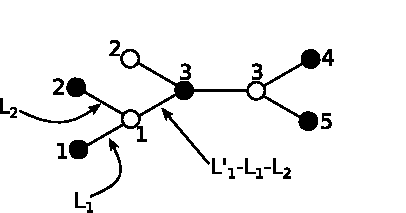
\includegraphics[width=0.3\textwidth]{tree-4.pdf}
    \end{itemize}
    \begin{figure}
        \centering
        \vspace{-8mm}
        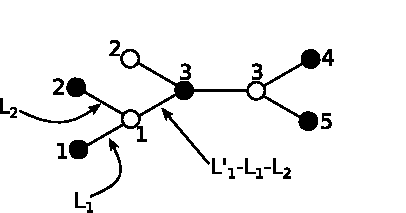
\includegraphics[width=0.4\textwidth]{tree-4.pdf}
        \vspace{-3mm}
    \end{figure}
    \begin{itemize}
        \item $g>0$: reduce to case $g=0$ using the bijection of \alert{Chapuy-F\'{e}ray-Fusy '13} between 1-face maps and decorated plane trees, via \alert{vertex explosions}.
    \end{itemize}
    \begin{figure}
        \centering
        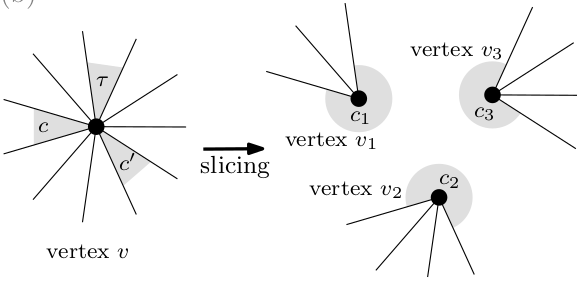
\includegraphics[height=0.3\textheight]{chapuy-2.png}
        \hspace{15mm}
        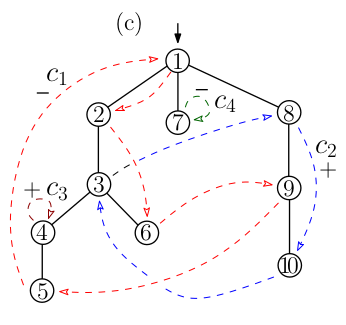
\includegraphics[height=0.3\textheight]{chapuy-3.png}
    \end{figure}
    % \begin{itemize}
    %     \item<2-> $\Pc^{[2(k+l-1)]}_{0,(k,l)}(L;L')$ is piecewise constant; by duality, it counts bipartite metric plane trees with fixed sums of lengths around each vertex (given by $L_i, L'_i$);
    %     \item<3-> each tree contributes either $1$ or $0$;
    %     \item<4-> when traversing a wall, we ``loose'' and ``gain'' an equal number of trees.
    % \end{itemize}
    % \begin{figure}
    % \begin{overprint}
    %     \onslide<1>
    %     \centering
    %     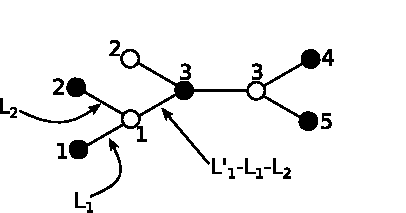
\includegraphics[width=0.4\textwidth]{tree-4.pdf}
    %     \hspace{0.4\textwidth}
    %     \onslide<4->
    %     \centering
    %     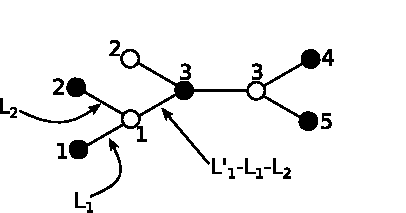
\includegraphics[width=0.4\textwidth]{tree-4.pdf}
    %     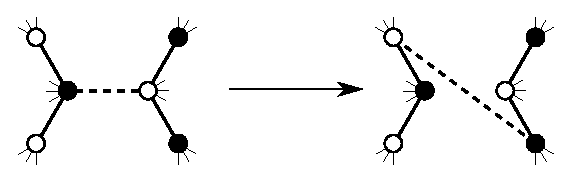
\includegraphics[width=0.4\textwidth]{bijection.eps}
    % \end{overprint}
    % \end{figure}
\end{frame}

% \begin{frame}{One-vertex face-bicolored graphs}
%     Sketch of proof ($g>0$):
%     \begin{itemize}
%         \item<2-> by duality, 1-face metric ribbon graphs with fixed sums of lengths around each vertex;
%         \item<3-> \textbf{Chapuy-F\'{e}ray-Fusy '13}: bijection between 1-face maps and decorated plane trees, via \alert{vertex explosions};
%         \item<4-> allows to control the metric!
%     \end{itemize}
    
%     \begin{figure}
%     \begin{overprint}
%         \onslide<3->
%         \centering
%         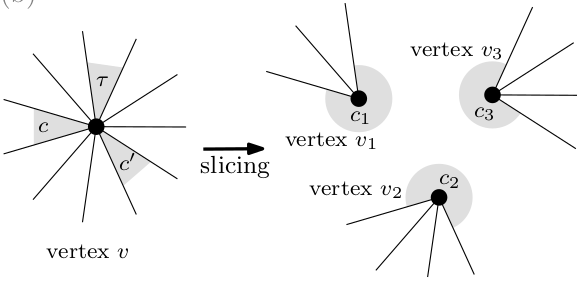
\includegraphics[height=0.3\textheight]{chapuy-2.png}
%         \hspace{15mm}
%         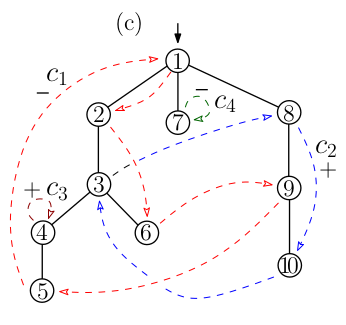
\includegraphics[height=0.4\textheight]{chapuy-3.png}
%     \end{overprint}
%     \end{figure}
% \end{frame}

\begin{frame}{NEW: many-vertex face-bicolored graphs}
    If there are $\ge 2$ vertices, even the top-degree term are \emph{not} polynomial... 
    
    \pause 
    Solution: \alert{weight} the contribution of each graph!

    \begin{figure}
        \begin{overprint}
            \onslide<3>
            \centering
            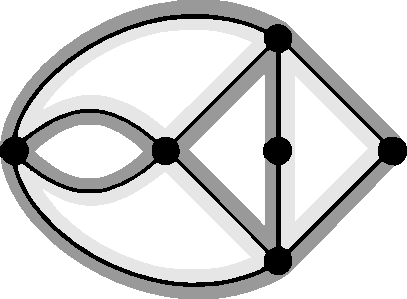
\includegraphics[width=0.25\textwidth]{weghting-1.pdf}
            \onslide<4>
            \centering
            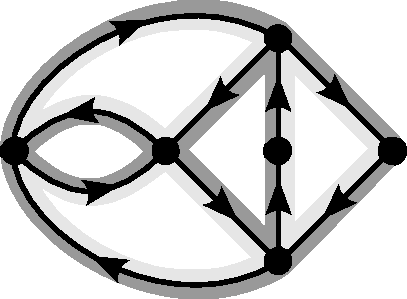
\includegraphics[width=0.25\textwidth]{weghting-2.pdf}
            \onslide<5->
            \centering
            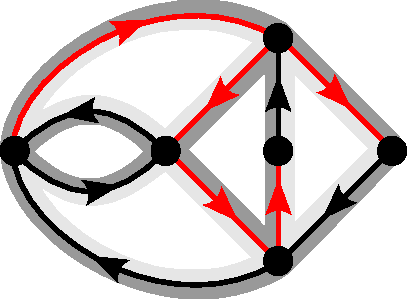
\includegraphics[width=0.25\textwidth]{weghting-3.pdf}
        \end{overprint}
    \end{figure}
    
    \begin{itemize}
    \pause \pause
        \item Orient each edge of $G$ so that the black face is to the left;
    \pause
        \item let $t(G)$ be the number of oriented spanning trees of $G$ rooted at an arbitrary vertex (independent of the vertex!);
    \end{itemize}
    \pause
    \begin{equation*}
    \widetilde{\mathcal{N}}^{d}_{g,(k,l)}(L,L') = \sum_{G \in \RGc^{d}_{g,(k,l)}} \frac{\alert{t(G)}}{|\operatorname{Aut}(G)|} \cdot \mathcal{N}_G(L,L').
    \end{equation*}
\end{frame}

\begin{frame}{NEW: many-vertex face-bicolored graphs}

    \begin{block}{Theorem (Y. '24)}
        For $g=0$, the \alert{top-degree term} of $\widetilde{\mathcal{N}}^{d}_{0,(k,l)}$ is a \alert{polynomial}
        \vspace{-2mm}
        \begin{equation*}
            (k+l-2)! \cdot (L_1+\ldots+L_k)^{\ell(d)-1}.
        \end{equation*}
    \end{block}

\pause
Idea: use the bijection of \alert{Bernardi '07} between tree-rooted plane maps and pairs of plane trees + more tricks with trees. %; refined enumeration of metric plane trees.

\begin{figure}
    \begin{overprint}
        \onslide<2> 
        \centering
        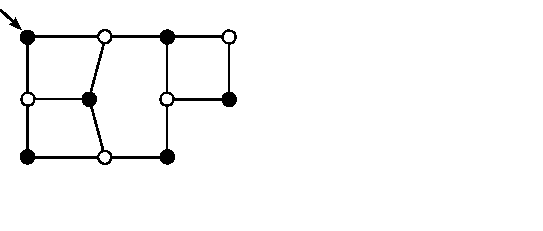
\includegraphics[width=0.6\textwidth]{many-vertices-bij.pdf}
        \onslide<3> 
        \centering
        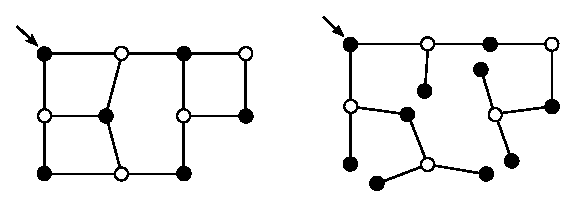
\includegraphics[width=0.6\textwidth]{many-vertices-bij-2.eps}
        \onslide<4-> 
        \centering
        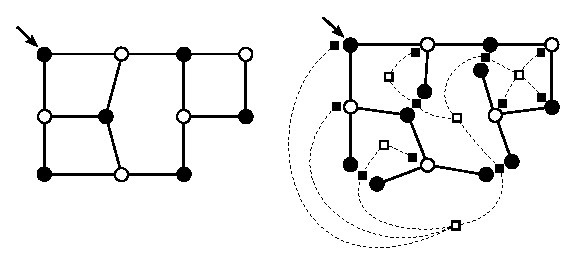
\includegraphics[width=0.6\textwidth]{many-vertices-bij-3.eps}
    \end{overprint}
\end{figure}

% \pause
%     \begin{block}{Conjecture}
%         Outside of the walls, the top-degree term of $\widetilde{\mathcal{P}}^{d}_{g,(k,l)}$ is a \alert{polynomial}
%         \vspace{-2mm}
%         \begin{equation*}
%             top\left( \Pc^{[2(k+l-1+2g)]}_{g,(k,l)} \right)(L,L') \cdot (L_1+\ldots+L_k)^{\ell(d)-1}. 
%         \end{equation*}
%     \end{block}
\end{frame}

\begin{frame}{Discussion}
    \begin{itemize}
        \item Weighted version is also true for $g>0$, but hard to prove bijectively.%(covered  maps of Bernardi-Chapuy '11)
        \pause
        \item From Kontsevich's proof one can also get a weighted version for trivalent graphs; weight = number of \alert{Kasteleyn orientations} with fixed ``indegrees''.
        \pause
        \item Formula $(k+l-2)! \cdot (L_1+\ldots+L_k)^{\ell(d)-1}$ suggests a double counting argument: each tree contributes $(L_1+\ldots+L_k)^{\ell(d)-1}$.
        \pause 
        \item It would be interesting to have such an argument for trivalent graphs \\$\Rightarrow$ combinatorics of the numbers $\int_{\overline{\Mc}_{g,n}} \psi_1^{\alpha_1}\cdots \psi_n^{\alpha_n}$.
    \end{itemize}
\end{frame}

% \begin{frame}{Graphs with odd vertex degrees}
%     \textbf{Kontsevich '92}: for any partition $d$ with odd parts, the top-degree term of $\Nc^d_{g,n}$ is a polynomial \emph{outside of the walls}.

% \pause
%     \begin{block}{Theorem (Duryev, Goujard, Y. '23)}
%         The top-degree term of $\Nc^d_{g,n}$ is also polynomial on any intersection of walls. \\
%         + Explicit recursive formula.
%     \end{block}
    
% \pause
%     \emph{Idea of proof}: 
%     \begin{itemize}
%         \item \alert{degeneration} of ribbon graphs on the walls (zero-length edges);
%         \item $\Rightarrow$ non-degenerated ribbon graphs glued into a tree-like structure;
%         \item count of the number of valid gluings.
%     \end{itemize} 
% \end{frame}

% \section{Applications to square-tiled surfaces / Masur-Veech volumes}

% % \begin{frame}{Square-tiled (ST) surfaces}

% %     \begin{figure}
% %         \centering
% %         \begin{minipage}{.45\textwidth}
% %             \centering
% %             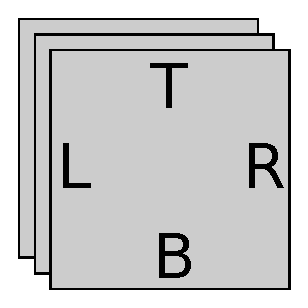
\includegraphics[height=0.25\textheight]{squares.eps}
% %             \caption{Gluing rule: $T \leftrightarrow B$, $L \leftrightarrow R$}
% %         \end{minipage}%
% %         \begin{minipage}{.45\textwidth}
% %         \pause
% %             \centering
% %             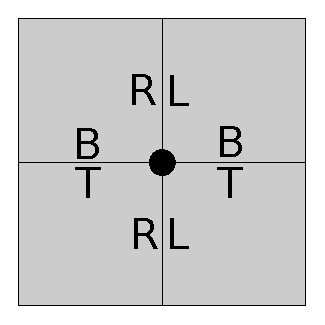
\includegraphics[height=0.25\textheight]{lightning_talk2.eps}
% %             \hspace{0.1\textwidth}
% %             %\pause 
% %             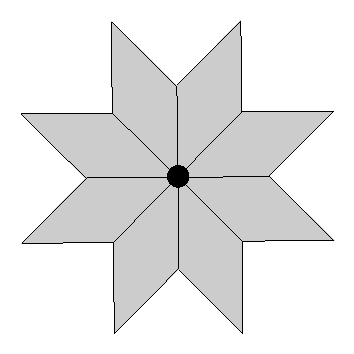
\includegraphics[height=0.25\textheight]{lightning_talk3.eps}
% %             %\vspace{0.05\textheight}
% %             \caption{\hspace{5mm} Local picture around a vertex. \\ \hspace{5mm} Singularity $\iff$ degree $>4$
% %             %\\ (labels are part of the data!)
% %             }
% %         \end{minipage}%
% %         \begin{minipage}{.1\textwidth}
% %             %\centering
% %             $\ldots$
% %         \end{minipage}%
% %     \end{figure}
% %     % \begin{figure}
% %     %         \centering
% %     %     \begin{minipage}{.5\textwidth}
% %     %         \centering
% %     %         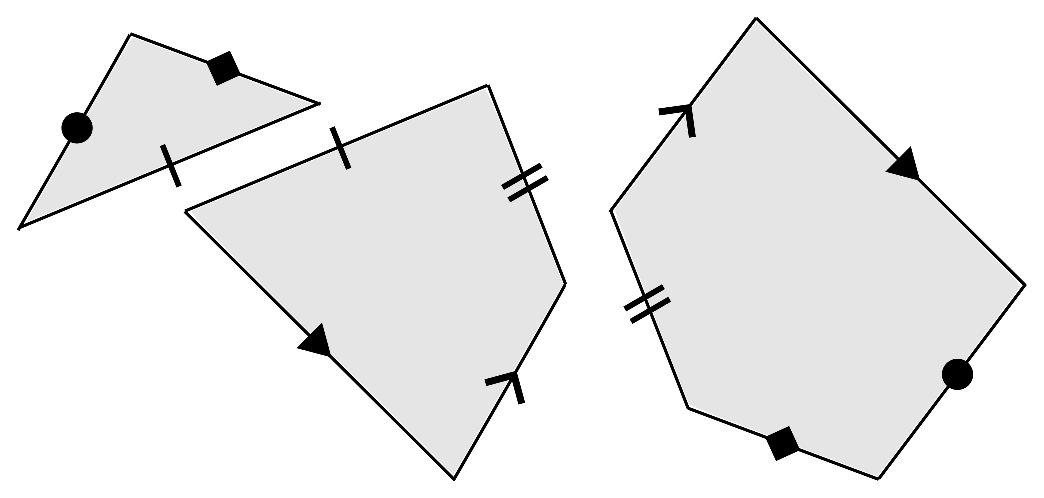
\includegraphics[height=0.25\textheight]{euclidean-polygons.eps}%
% %     %         \caption{ST surfaces $\subset$ translation surfaces}%
% %     %     \end{minipage}%
% %     %     \begin{minipage}{.5\textwidth}
% %     %         \centering
% %     %         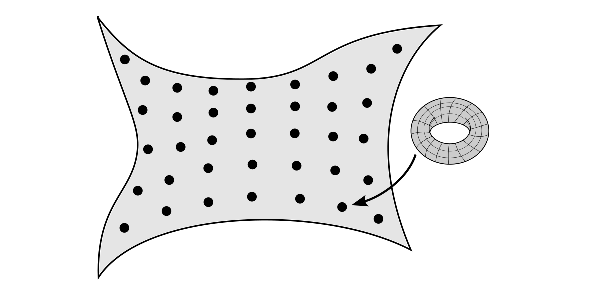
\includegraphics[height=0.25\textheight]{moduli-2.eps}
% %     %         \caption{Asymptotic enumeration of $\mathcal{ST}(k)$ $\iff$ \emph{Masur-Veech} volume of the stratum $\mathcal{H}(k)$
% %     %         }
% %     %     \end{minipage}
% %     % \end{figure}

% % \pause
% %     \begin{equation*}
% %         \# \left \{ 
% %     \begin{array}{c}
% %          \text{ST surfaces with given degrees of }\\ \text{singularities } d_i          \text{ and } \leq N \text{ squares}
% %     \end{array} \right \}
% %     \sim c(d) \cdot N^{D(d)}.%,\ N \rightarrow \infty.
% %     \end{equation*}

% % \pause
% %     $c(d)$ -- \alert{Masur-Veech volume} of the corresponding \emph{stratum of translation surfaces}.
% % \end{frame}

% % % \begin{frame}{Square-tiled (ST) surfaces}

% % %     \begin{figure}
% % %         \centering
% % %         \begin{minipage}{.45\textwidth}
% % %             \centering
% % %             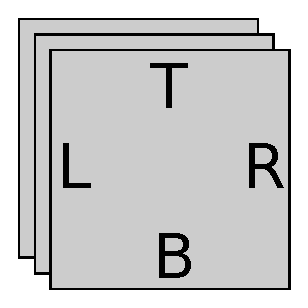
\includegraphics[height=0.25\textheight]{squares.eps}
% % %             \caption{Gluing rule: $T \leftrightarrow B$, $L \leftrightarrow R$}
% % %         \end{minipage}%
% % %         \begin{minipage}{.1\textwidth}
% % %             %\centering
% % %             $\longrightarrow$
% % %         \end{minipage}%
% % %         \begin{minipage}{.45\textwidth}
% % %             \centering
% % %             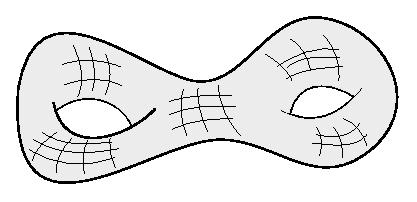
\includegraphics[height=0.2\textheight]{surface.eps}
% % %             \vspace{0.05\textheight}
% % %             \caption{Oriented, closed surface
% % %             %\\ (labels are part of the data!)
% % %             }
% % %         \end{minipage}

        
% % %     \end{figure}
    
% % %     \begin{itemize}
% % %         \item Local picture around a vertex:
% % %     \end{itemize} 

% % %     \begin{figure}
% % %         \centering
% % %         \begin{minipage}{.5\textwidth}
% % %             \centering
% % %             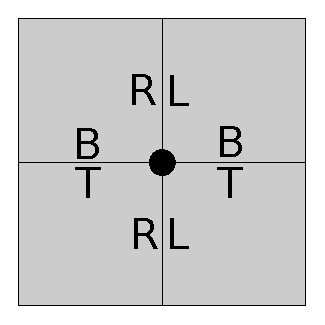
\includegraphics[height=0.25\textheight]{lightning_talk2.eps}
% % %             \hspace{0.1\textwidth}
% % %             %\pause 
% % %             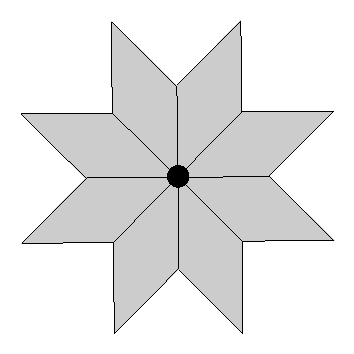
\includegraphics[height=0.25\textheight]{lightning_talk3.eps}
% % %         \end{minipage}%
% % %         \begin{minipage}{.5\textwidth}
% % %             ... $\Rightarrow$ all degrees are multiples of 4.
% % %         \end{minipage}
% % %     \end{figure}
% % % \end{frame}


% % % \begin{frame}{ST surfaces $\subset$ translation surfaces}
% % %     Suppose that the squares are euclidean unit squares. 
    
% % %     A ST surface then becomes a \emph{flat surface with conical singularities} (of angles $2\pi(k_i+1)$) \emph{and with trivial holonomy} =: \alert{translation surface}.

% % %     \begin{figure}
% % %         \centering
% % %         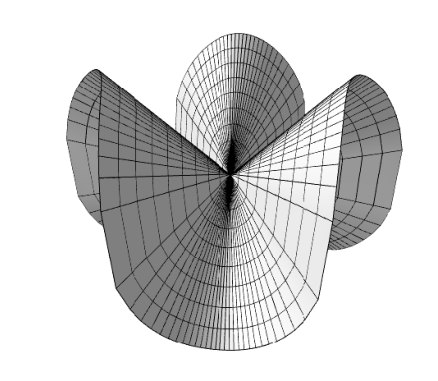
\includegraphics[height=0.3\textheight]{singularity.eps}
% % %         \hspace{1cm}
% % %         %\pause 
% % %         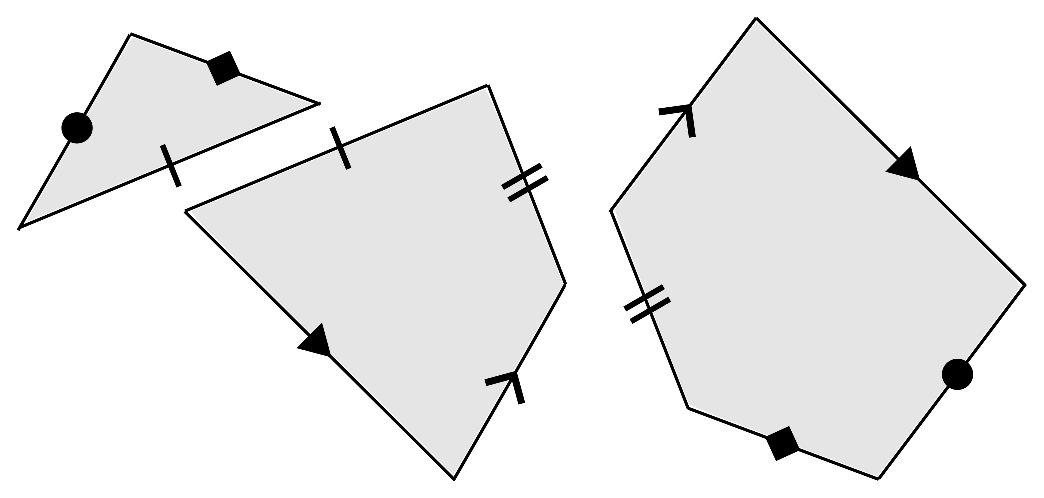
\includegraphics[height=0.3\textheight]{euclidean-polygons.eps}
% % %     \end{figure}
    
% % %     Gluings of \emph{arbitrary} euclidean polygons along equal and parallel sides.
% % % \end{frame}

% % % \begin{frame}{ST surfaces $\subset$ translation surfaces}

% % % \begin{figure}
% % %         \centering
% % %         \begin{minipage}{.5\textwidth}
% % %             \begin{overprint}
% % %             \onslide<1>
% % %             \begin{figure}
% % %                 \centering
% % %                 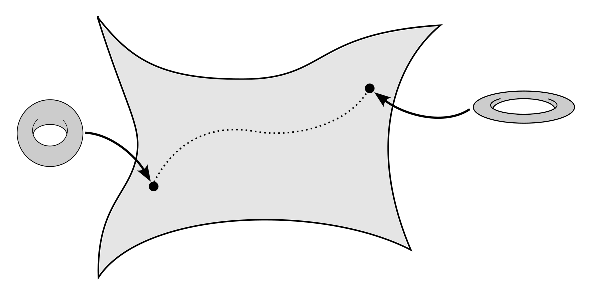
\includegraphics[height=0.3\textheight]{moduli-1.eps}
% % %                 \caption{}
% % %             \end{figure}
% % %             \onslide<2-3>
% % %             \begin{figure}
% % %                 \centering
% % %                 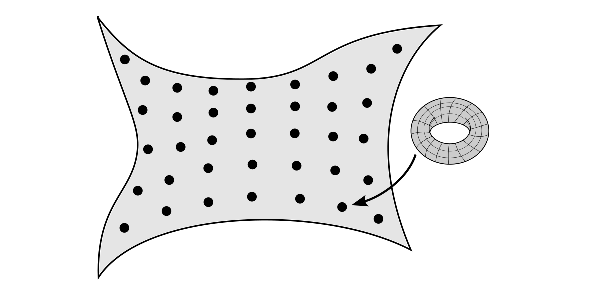
\includegraphics[height=0.3\textheight]{moduli-2.eps}
% % %                 \caption{$\mathcal{ST}(k) \subset \mathcal{H}(k)$}
% % %             \end{figure}
% % %             \end{overprint}
% % %         \end{minipage}%
% % %         \begin{minipage}{.5\textwidth}
% % %             \begin{overprint}
% % %             \onslide<3>
% % %                 \begin{figure}
% % %                 \centering
% % %                 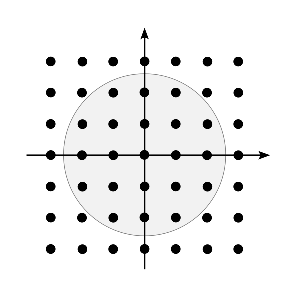
\includegraphics[height=0.3\textheight]{moduli-3.eps}
% % %                 \caption{$\mathbb{Z}^n \subset \mathbb{R}^n$}
% % %                 \end{figure}
% % %             \end{overprint}
% % %         \end{minipage}
% % %     \end{figure}

% % % \begin{itemize}
% % %     \item<1-3> Translation surfaces come in continuous families, called \emph{strata} $\mathcal{H}(k)$, parametrized by the angles of singularities $k$. %These are orbifolds with rich topology, geometry and dynamics.
% % %     \item<2-3> ST surfaces are ``integer points'' of strata!
% % %     \item<3> Asymptotic enumeration of $\mathcal{ST}(k)$ $\iff$ computing the volume of the ``unit ball'' in $\mathcal{H}(k)$ for the (natural) \emph{Masur-Veech measure}.
% % % \end{itemize}
% % % \end{frame}

% % \begin{frame}{Masur-Veech volumes}

% % Generating series / recursions were obtained in the works of \textbf{Chen, M\"{o}ller, Sauvaget and Zagier '18, '20} via \emph{algebraic geometry} (intersection numbers).
% % \smallskip

% % \pause
% % \textbf{Delecroix-Goujard-Zograf-Zorich '21}: combinatorial formula for the volumes of \emph{principal} strata of \emph{half}-translation surfaces, using \alert{cylinder decomposition} of STS.\smallskip
% %     % \begin{figure}
% %     %     \centering
% %     %     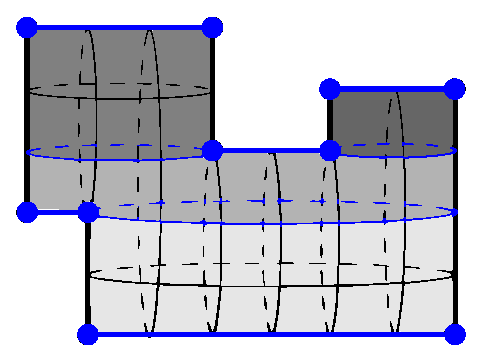
\includegraphics[height=0.3\textheight]{square-tiled-cartoon-3.eps}
% %     %     \hspace{5mm}
% %     %     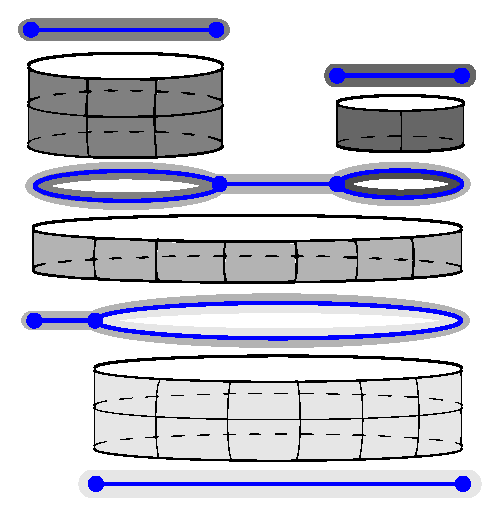
\includegraphics[height=0.3\textheight]{square-tiled-cartoon-4.eps}

% %     %     $\Rightarrow$ \emph{trivalent} metric ribbon graphs $\Rightarrow$ Kontsevich polynomials.
% %     % \end{figure}

% % %Applications: large genus asymptotics of volumes, properties of random square-tiled surfaces / random geodesic multicurves on hyperbolic surfaces.

% % \pause
% % Motivation: extend this strategy to strata of \emph{translation} surfaces.
% % \pause

% %     \begin{figure}
% %         \begin{overprint}
% %             \onslide<4>
% %             \centering
% %             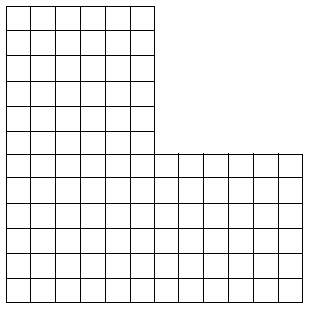
\includegraphics[height=0.4\textheight]{st-example-1.pdf}
% %             \hspace{18.4mm}\hspace{0.4\textwidth}
% %             \onslide<5>
% %             \centering
% %             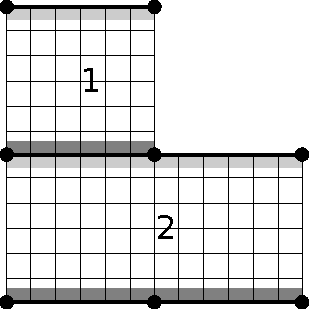
\includegraphics[height=0.4\textheight]{st-example-2.pdf}
% %             \hspace{18.4mm}\hspace{0.4\textwidth}
% %             \onslide<6>
% %             \centering
% %             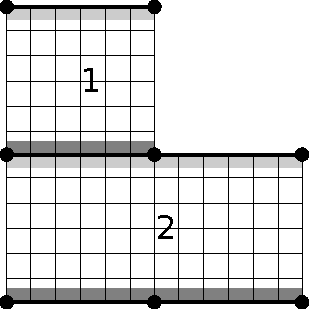
\includegraphics[height=0.4\textheight]{st-example-2.pdf}
% %             \hspace{2cm}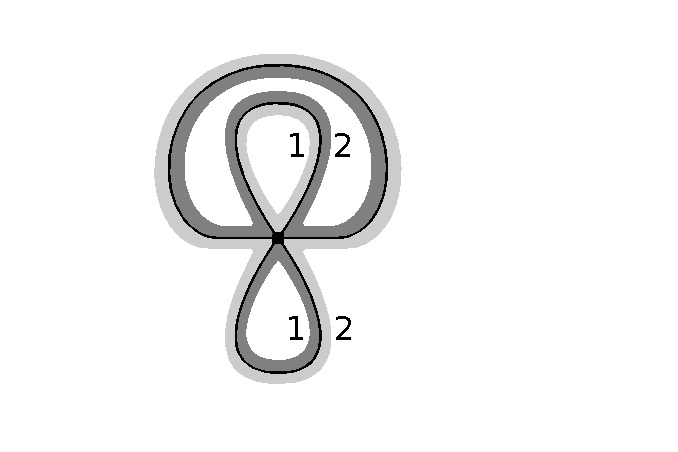
\includegraphics[height=0.4\textheight]{ribbon_graph_to_st-0.pdf}
% %             \onslide<7->
% %             \centering
% %             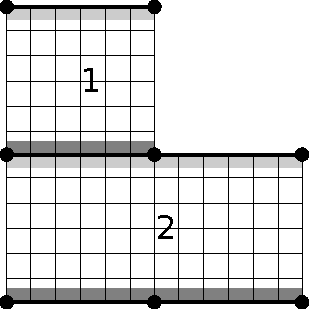
\includegraphics[height=0.4\textheight]{st-example-2.pdf}
% %             \hspace{2cm}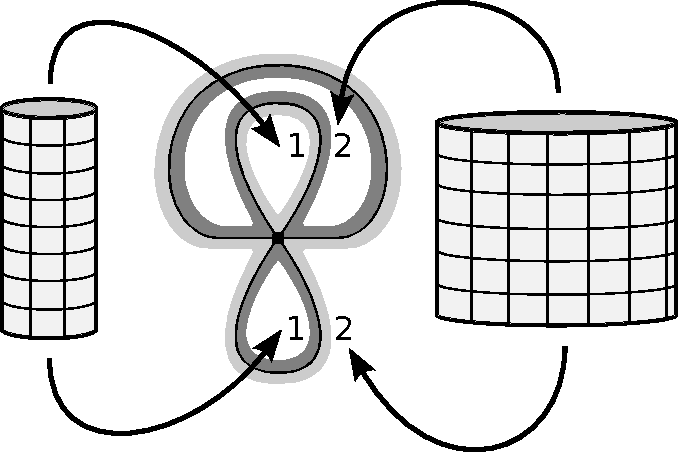
\includegraphics[height=0.4\textheight]{ribbon_graph_to_st-1.pdf}
            
% %             $\Rightarrow$ \emph{face-bicolored} metric ribbon graphs.
% %         \end{overprint}
% %     \end{figure}

% % \end{frame}


% \begin{frame}{Minimal strata}
%     Using our result on one-vertex face-bicolored graphs, we get:
    
% \pause
%     \begin{block}{Theorem (Y. '23)}
%     The contribution of $n$-cylinder square-tiled surfaces to the volume of the minimal stratum $\mathcal{H}(2g-2)$ is equal to $\frac{2(2\pi)^{2g}}{(2g-1)!}a_{g,n}$, where $a_{g,n}\in \Qm$ and whose generating function $\mathcal{C}(t,u) = 1 + \sum_{g\geq 1} \left(\sum_{n=1}^g a_{g,n} u^n \right) (2g-1)t^{2g}$ satisfies for all $g\ge 0$
%     \[
%     \frac{1}{(2g)!} [t^{2g}] \mathcal{C}(t,u)^{2g} = [t^{2g}] \left(\frac{t/2}{\sin(t/2)}\right)^u.
%     \]
%     \end{block}
%     \begin{itemize}
%     \pause
%         \item Lagrange inversion $\Rightarrow$ explicit formula for $\mathcal{C}(t,u)$;
%     \pause
%         \item setting $u=1$ we recover the result of \textbf{Sauvaget '18}.
%     \pause
%         \item \textbf{Faber-Pandharipande '00}: $\left(\frac{t/2}{\sin(t/2)}\right)^{u+1}$ is the generating function of Hodge integrals $\int_{\overline{\mathcal{M}}_{g,1}} \lambda_{g-i} \psi_1^{2g-2+i}$
%     \end{itemize}
% \end{frame}

% \begin{frame}{Odd strata of half-translation surfaces}
%     Using our result on graphs with odd vertex degrees, we get:
% \pause
%     \begin{block}{Theorem (Duryev, Goujard, Y. '23)}
%         Formula for the ``completed'' volume of any odd stratum, in terms of intersection numbers of $\psi$-classes and Kontsevich-Witten combinatorial classes.
%     \end{block}

%     \begin{itemize}
%     \pause
%         \item \alert{``Completed volume''} $=$ volume $+$ weighted sum of volumes of some (smaller) adjacent strata.
%     \pause
%         \item \textbf{Di Francesco-Itzykson-Zuber '93}: expression for intersection numbers in question in terms of intersection numbers of $\psi$-classes.
%     \end{itemize}
    
% \end{frame}
% \section{Conclusion}

% \begin{frame}{Recap and open questions}

%     \begin{itemize}
%         \item \emph{Polynomiality of the top-degree term}: one-vertex face-bicolored, many-vertex face-bicolored (weighted), odd vertex degrees (on the walls).
%         \item \emph{Applications to Masur-Veech volumes}: cylinder contributions in minimal strata, completed volumes of odd strata of half-translation surfaces.
%     \end{itemize}

%     % Polynomiality of the top-degree term:
%     % \begin{itemize}
%     %     \item one-vertex face-bicolored graphs;
%     %     \item weighted version for planar many-vertex face-bicolored graphs;
%     %     \item graphs with odd vertex degrees, on the walls.
%     % \end{itemize}
%     % Applications to Masur-Veech volumes: 
%     % \begin{itemize}
%     %     \item cylinder contributions in minimal strata of translation surfaces;
%     %     \item completed volumes of odd strata of half-translation surfaces.
%     % \end{itemize} 
%     \smallskip
%     \pause
%     Open questions:
%     \begin{itemize}
%         \item cylinder contributions in spin connected components of minimal strata;
%         \item large genus asymptotics of cylinder contributions;
%         \item algebraic geometry interpretation;
%         %\item non-minimal strata?
%         \item study Kontsevich polynomials combinatorially.
%     \end{itemize}
% \end{frame}


% %%%%%%%%%%%%%%%%%%%%%%%%%%%%%%%%%%%%


% % \begin{frame}{Computing counting functions on the walls}
% %     When passing to an intersection of walls, certain ribbon graphs \emph{degenerate}: some of their bridges become zero-length.

% %     Such ribbon graphs decompose into positive pieces forming a tree-like structure.

% %     The pieces are enumerated by the counting functions with smaller parameters.

% %     It suffices to count the number of degenerations producing a fixed set of pieces.
% % \end{frame}



% % \begin{frame}{Computing counting functions on the walls}
% %     Idea: choose a specific direction from which to degenerate $\Rightarrow$ specific structure of degenerations.

% % Bipartite case: 

% % Direction: $\left(L_1+(k-1)\varepsilon, L_2-\varepsilon, \ldots, L_k-\varepsilon; L'_1, \ldots, L'_k \right),\  \varepsilon \rightarrow 0, \varepsilon > 0$

% % Structure: Zero-length edges are oriented with their black extremity towards the tree containing vertex 1.

% % Non-bipartite case:

% % Direction: $(L_1)$
    
% % \end{frame}
% % %----------------------------------------------------

% % %\section{One-vertex graphs}

% % \begin{frame}{One-vertex graphs}
% %      \begin{figure}
% %         \centering
% %         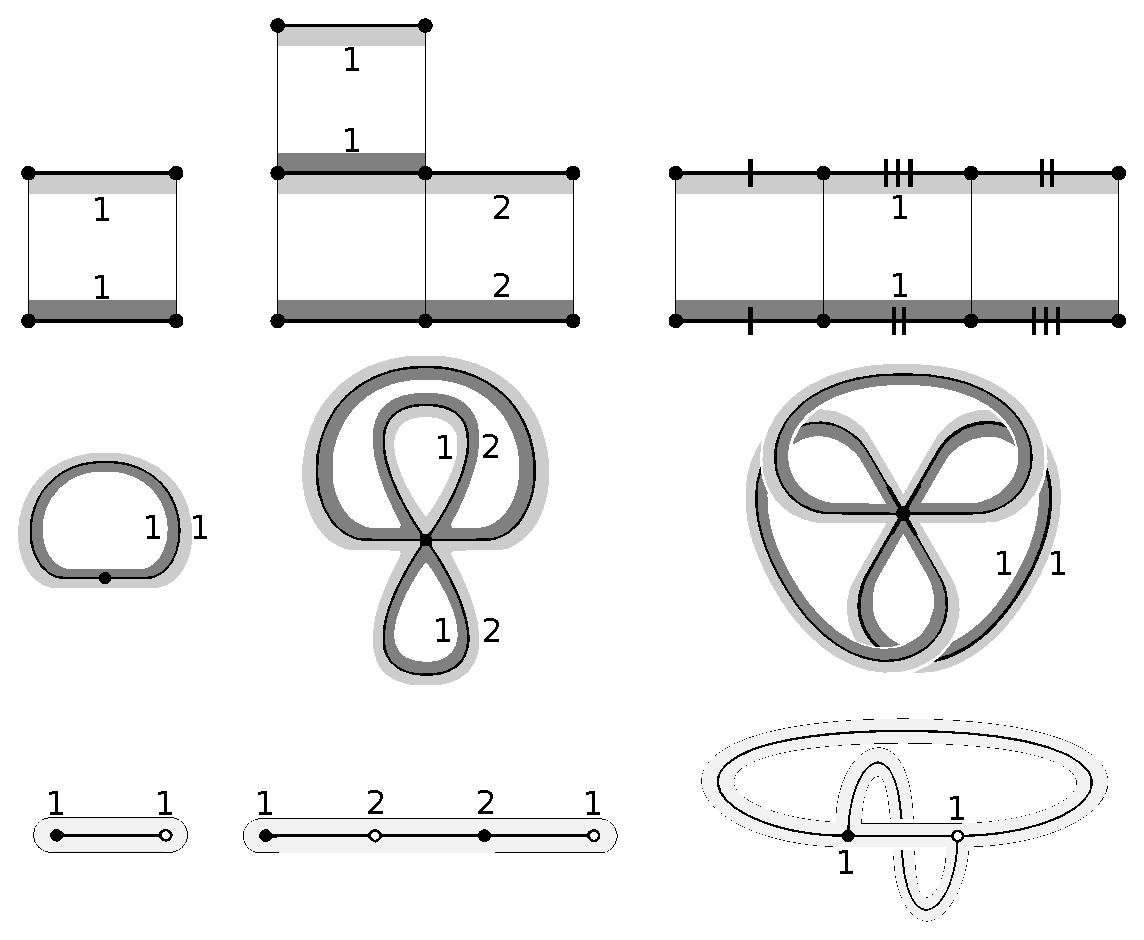
\includegraphics[trim={0cm 4cm 0 5.5cm},clip,width=0.8\textwidth]{examples.eps}
% %     \end{figure}

% %     Since there is just one vertex, we omit $v$ from the notation: $\mathcal{P}^{g}_{k,l}(L;L').$
% % \end{frame}

% % \begin{frame}{A result on $\mathcal{P}^{g}_{k,l}$}
% %     Consider the cone $C_{k,l} = \mathbb{R}_{>0}^{k+l} \cap \{L_1+\ldots+L_k=L'_1+\ldots+L'_l\}$. 
    
% %      It is sliced by the ``walls'' given by equations of type $\sum_{i \in I} L_i = \sum_{j \in J} L'_j$.
% %     \begin{figure}
% %         \centering
% %         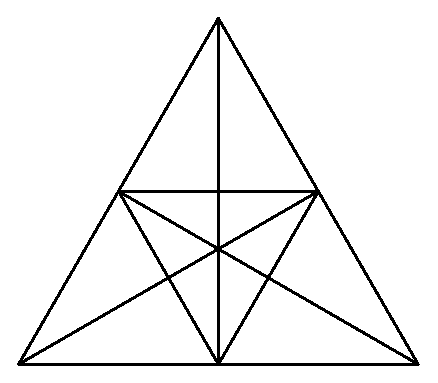
\includegraphics[height=0.3\textheight]{walls.eps}
% %     \end{figure}
    
% %      \begin{theorem}[Y., 2023]
% %     On $C_{k,l}$ and outside of the walls, $top(\mathcal{P}^g_{k,l})$ is a \textbf{polynomial} of degree $2g$. 
% %     \end{theorem}
    
% %      The same statement is true on the intersection of any subset of walls. 
    
% %     The coefficients of all polynomials are explicit.
    
% % \end{frame}


% % \begin{frame}{Proof outline}
% %      Pass to the dual ribbon graph:

% %     \begin{figure}
% %         \centering
% %         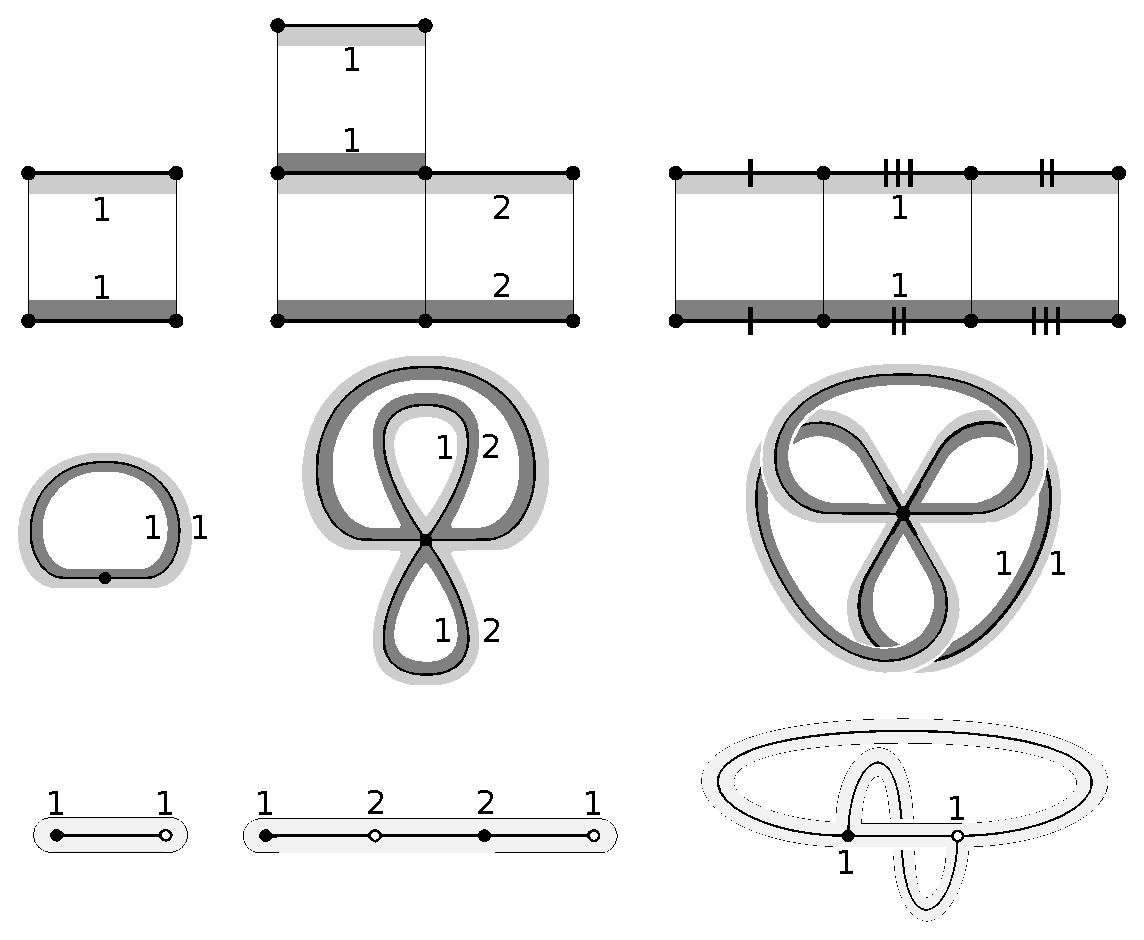
\includegraphics[trim={0cm 0cm 0 5.5cm},clip,width=0.6\textwidth]{examples.eps}
% %     \end{figure}
    
% %      Then $\mathcal{P}^{g}_{k,l}$ counts metric ribbon graphs with 1 boundary (=\emph{unicellular maps}), vertex-bicolored, with prescribed sums of edge lengths around each vertex.
% % \end{frame}

% % \begin{frame}{Case $g=0$: metric plane trees}
% %     \begin{lem}
% %         There is at most one metric on a planar tree with given sums $L, L'$ of edge lengths around every vertex. Moreover, the edge lengths are linear functions of $L, L'$ of the form  $\sum_{i \in I} L_i - \sum_{j \in J} L'_j$.
% %     \end{lem}
% %      \emph{Proof:}    
% %         \begin{overprint}
% %             \onslide<1>
% %             \begin{center}
% %             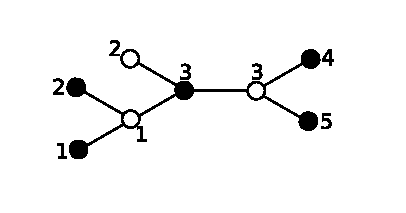
\includegraphics[height=0.4\textheight]{tree-1.pdf}
% %             \end{center}
% %             \onslide<2>
% %             \begin{center}
% %             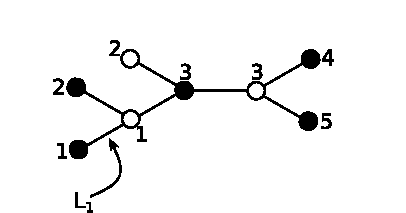
\includegraphics[height=0.4\textheight]{tree-2.pdf}
% %             \end{center}
% %             \onslide<3>
% %             \begin{center}
% %             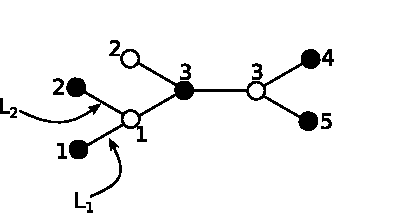
\includegraphics[height=0.4\textheight]{tree-3.pdf}
% %             \end{center}
% %             \onslide<4>
% %             \begin{center}
% %             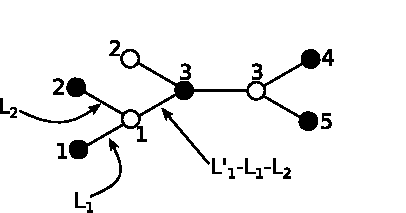
\includegraphics[height=0.4\textheight]{tree-4.pdf}
% %             \end{center}
% %             \onslide<5>
% %             \begin{center}
% %             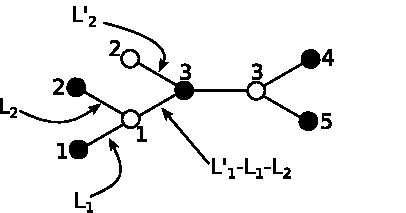
\includegraphics[height=0.4\textheight]{tree-5.pdf}
% %             \end{center}
% %             \onslide<6>
% %             \begin{center}
% %             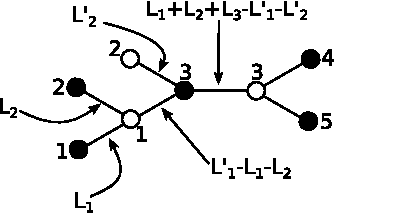
\includegraphics[height=0.4\textheight]{tree-6.pdf}
% %             \end{center}
% %             %\onslide<7>
% %             %\begin{center}
% %             %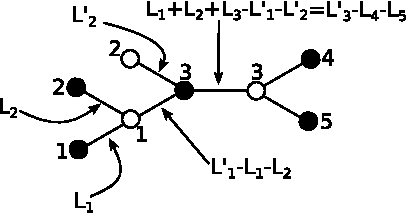
\includegraphics[height=0.4\textheight]{tree-7.pdf}
% %             %\end{center}
% %             This is a metric $\iff$ all linear forms are positive! \qed
% %         \end{overprint}
% % \end{frame}

% % \begin{frame}{Case $g=0$: metric plane trees}
% %     Lemma $\Rightarrow$ $\mathcal{P}^0_{k,l}(L;L')$ is constant outside of the walls.
% %      \begin{prop}
% %         When the point $(L;L')$ traverses a wall, the value of $\mathcal{P}^0_{k,l}(L;L')$ does not change. 
% %     \end{prop}
% %      \emph{Proof:}
% %     \begin{figure}
% %         \centering
% %         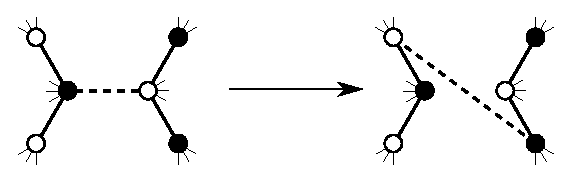
\includegraphics[height=0.2\textheight]{bijection.eps}
% %     \end{figure}
% %     \qed

% %      Thus $\mathcal{P}^0_{k,l}(L;L')$ is constant outside the walls.
% % \end{frame}

% % \begin{frame}{Case $g>0$: ideas}
% %     \begin{itemize}
% %          \item There is a bijection (due to Chapuy, F\'{e}ray, Fusy) between unicellular maps and plane trees decorated with certain permutation on the set of vertices;
% %         \begin{figure}
% %             \centering
% %             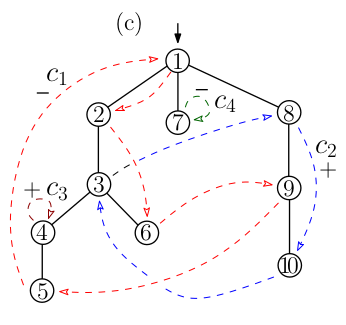
\includegraphics[height=0.4\textheight]{chapuy-3.png}
% %         \end{figure}
% %          \item to get the map, glue vertices in each cycle!
% %          \item $top(\mathcal{P}^g_{k,l})$ is the sum of \emph{volumes} of the corresponding polytopes;
% %          \item so $top(\mathcal{P}^g_{k,l})$ is the integral of $\mathcal{P}^0_{*,*}$ over simplices $\{x_3+x_8+x_{10}=L_2\}$, etc.
% %     \end{itemize}
% %     \qed
% % \end{frame}


% % %----------------------------------------------------
% % %\section{Spin parity}

% % \begin{frame}{A word about motivation}
% %      Polynomials $top(\mathcal{P}^g_{k,l})(L;L')$ with $k=l$ and $L_i=L'_i\in \mathbb{Z}$ for all $i$ are useful for \emph{asymptotic enumeration} of \emph{square-tiled surfaces with one singularity}.

% %      \begin{figure}
% %         \centering
% %         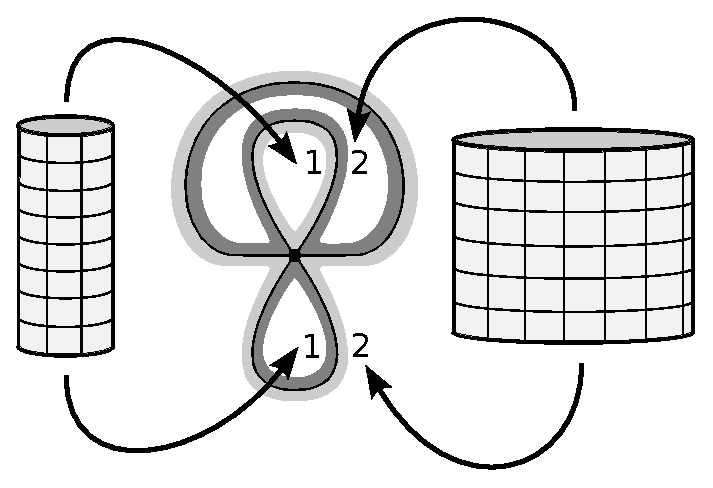
\includegraphics[height=0.4\textheight]{ribbon_graph_to_st.eps}
% %     \end{figure}
    
% %     To get a ST surface: for each $i$, glue a square-tiled cylinder of circumference $L_i$ to the two corresponding boundaries of the ribbon graph. 

% %     To come back: canonical decomposition into cylinders + ribbon graph.
    
    
    
% % \end{frame}

% % \begin{frame}{A word about motivation}
% %      Square-tiled surfaces live inside \emph{continuous} families of flat surfaces.

% %     \begin{figure}
% %         \centering
% %         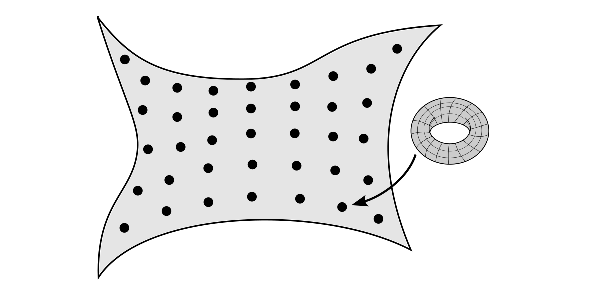
\includegraphics[height=0.3\textheight]{moduli-2.eps}
% %          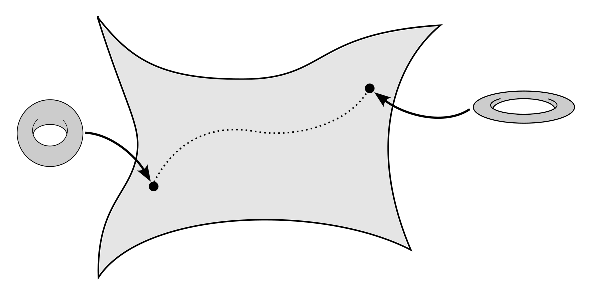
\includegraphics[height=0.3\textheight]{moduli-1.eps}
% %     \end{figure}
    
% %     Ribbon graphs with the same $g,k,l$ can give surfaces from different families (i.e. not connected by a continuous deformation).

% %      How to distinguish ribbon graphs of different types? Do these subfamilies of ribbon graphs enjoy a polynomiality property? $\Rightarrow$ enumerate ST surfaces in each continuous family?
% % \end{frame}

% % \begin{frame}{Spin parity}

% %     There is a topological invariant of flat surfaces (\emph{spin parity}) which can distinguish different families. What is the corresponding invariant of ribbon graphs?

% %      Hopefully, for plane trees this invariant is preserved by flips (otherwise our proof breaks down...)

% %      \begin{theorem}[Y.]
% %         \begin{itemize}
% %             \item If $k-l$ is odd, any two trees with $k$ black and $l$ white labeled vertices are connected by a sequence of flips.
% %             \item If $k-l$ is even, there are exactly 2 equivalence classes! The counting function for each class is constant outside the walls.
% %         \end{itemize}
% %     \end{theorem}
% % \end{frame}

% % \begin{frame}{Spin parity for plane trees}
% %      Are these two trees connected by flips?
% %     \begin{figure}
% %         \centering
% %         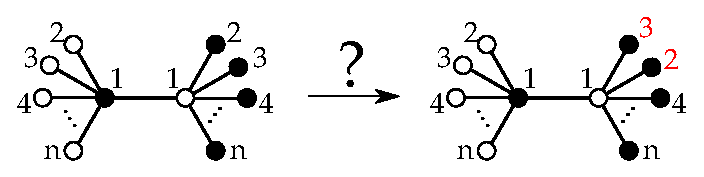
\includegraphics[height=0.2\textheight]{tree-question.eps}
% %     \end{figure}

% %      No! Choose a root, make a tour around your tree, record \emph{first} visits to black vertices and \emph{last} visits to white vertices (``prefix-postfix'' traversal). The parity of the obtained permutation is flip-invariant!

% %     \begin{figure}
% %         \centering
% %         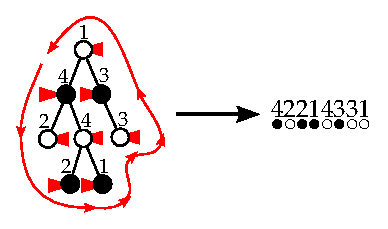
\includegraphics[height=0.32\textheight]{prefix-postfix.eps}
% %     \end{figure}
% % \end{frame}

% % \begin{frame}{Spin parity for $g>0$}
% %         \begin{conj}[work in progress]
% %         For any $g$, if $k-l$ is even, there is a partition of the corresponding ribbon graphs into 2 subfamilies such that the counting functions for each subfamily have polynomial top-degree terms.
% %     \end{conj}
% % \end{frame}

% % %----------------------------------------------------
% % %\section{Digression: triangulations of polytopes}

% % \begin{frame}{Flipping edges cleverly}
% %     \begin{claim}
% %     \begin{itemize}
% %         \item For any non-root edge in any (rooted) tree, there is a unique way to flip it so that the prefix-postfix sequence does not change!
% %         \item There is a unique way to flip the root edge so that the prefix-postfix sequence changes by a cyclic permutation.
% %     \end{itemize}
% %     \end{claim}

% %     \begin{figure}
% %         \centering
% %          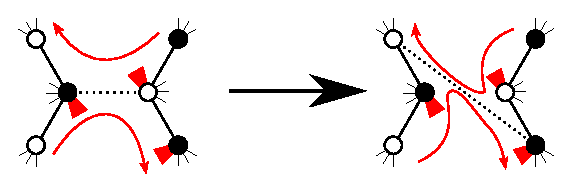
\includegraphics[width=0.45\textwidth]{clever-flip.eps}\hspace{5mm}
% %          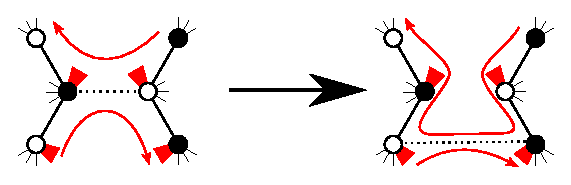
\includegraphics[width=0.45\textwidth]{clever-flip-2.eps}
% %     \end{figure}
% % \end{frame}

% % \begin{frame}{From trees to triangulations}
% %      Consider a subfamily $F$ of (rooted) trees with a given prefix-postfix sequence (modulo cyclic permutations).

% %     \begin{itemize}
% %          \item The counting function of $F$ is constant. One can show (by a simple counting argument) that it is in fact equal to 1!

% %          \item It means that for every point $(L;L')$ there is a unique tree $t\in F$ that contributes at this point.

% %          \item But each tree contributes on a simplicial cone (generated by its edges).

% %          \item Hence these cones form a simplicial decomposition of the ambient cone $C$.
% %     \end{itemize}

% %      Projectivizing, we get a triangulation of the polytope $\mathbb{P}C = \Delta_k \times \Delta_l$ -- the product of two simplices!

% % \end{frame}

% % \begin{frame}{Example for $k=l=3$}
% %     \begin{figure}
% %         \centering
% %         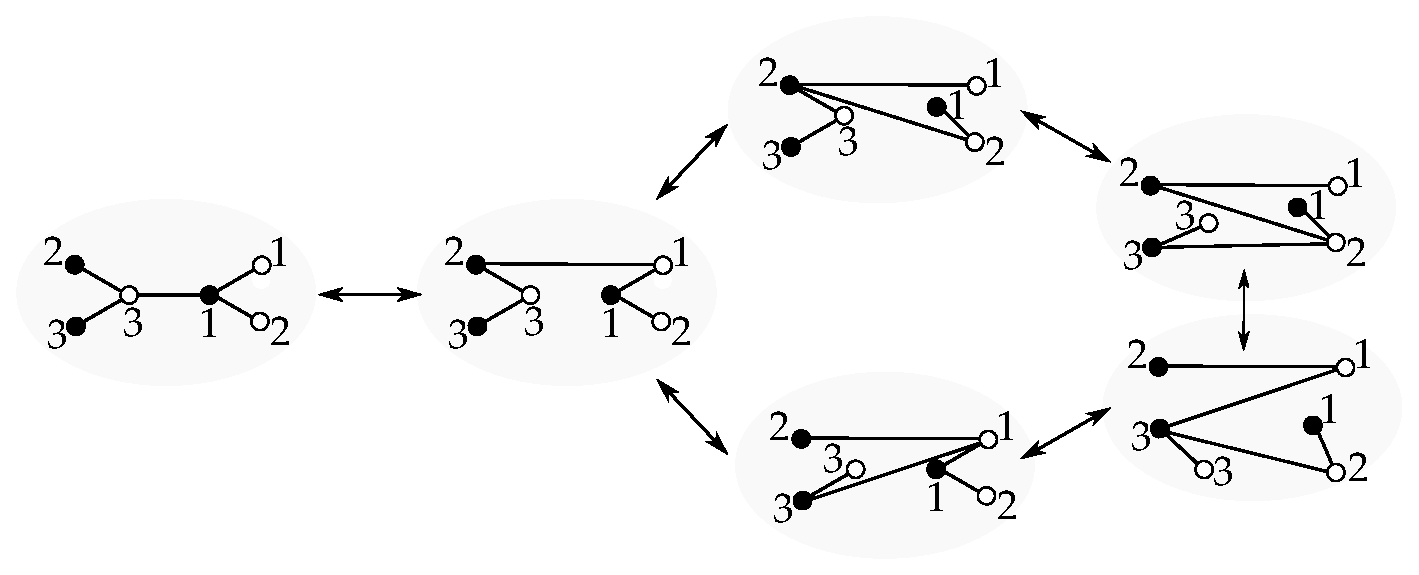
\includegraphics[width=0.95\textwidth]{triang-prod-simplices.eps}
% %     \end{figure} 
% % \end{frame}

% % %----------------------------------------------------
% % %\section{Many-vertex graphs}

% % \begin{frame}{Many-vertex graphs}
% %     \begin{itemize}
% %         \item When there are at least 2 vertices, even the top-degree term of $\mathcal{P}^{g,v}_{k,l}(L;L')$ is not polynomial. However...
% %         \item For any $g,v,k,l$ let $\overline{\mathcal{P}}^{g,v}_{k,l}(L;L')$ be the \emph{weighted} sum of contributions of corresponding graphs, where the weight $t(G)$ of a graph $G$ is defined as follows.
% %         \item Orient every edge of $G$ in such a way that the black adjacent boundary is on the left. Then $t(G)$ is the number of oriented spanning trees centered at any vertex (this number does not depend on the vertex!).
% %     \end{itemize}

% %     \begin{conj}[work in progress]
% %         The top-degree term of $\overline{\mathcal{P}}^{g,v}_{k,l}(L;L')$ is polynomial for all $g,v,k,l$.
% %     \end{conj}
    
    
    
    
% % \end{frame}

\end{document}
